\documentclass[a4paper,12pt,twoside,oldfontcommands]{memoir}


\usepackage[spanish,es-tabla]{babel}
\usepackage{imakeidx}
\usepackage[utf8]{inputenc}
\usepackage{amsmath}
\usepackage{graphicx}
\usepackage[T1]{fontenc}
\usepackage{lmodern} % scalable font
\usepackage{microtype}
\usepackage{placeins}
\usepackage{caption}
\usepackage{subcaption}
\usepackage[colorinlistoftodos]{todonotes}
\usepackage{listings}
\usepackage[hyphens]{url}

\RequirePackage{booktabs}
\RequirePackage{xtab}
\usepackage{longtable}
\usepackage[colorlinks]{hyperref}
\hypersetup{
	allcolors = {red}
} %Enlaces

%Parrafos
\nonzeroparskip

%Capítulos
\chapterstyle{bianchi}
% \newcommand{\capitulo}[2]{
% 	\setcounter{chapter}{#1}
% 	\setcounter{section}{0}
% 	\chapter*{#2}
% 	\addcontentsline{toc}{chapter}{#2}
% 	\markboth{#2}{#2}
% }

\usepackage[htt]{hyphenat} %Saltos de líneas en monoespaciados

%\renewcommand\thesection{\arabic{section}}


%PORTADA

% Formato de portada
\makeatletter
\usepackage{xcolor}
\newcommand{\tutor}[1]{\def\@tutor{#1}}
\newcommand{\course}[1]{\def\@course{#1}}
\definecolor{cpardoBox}{HTML}{E6E6FF}
\def\maketitle{
  \null
  \thispagestyle{empty}
  % Cabecera ----------------
\noindent
\includegraphics[width=\textwidth]{images/cabecera.pdf}\vspace{1cm}%
  \vfill
  % Título proyecto y escudo informática ----------------
  \colorbox{cpardoBox}{%
    \begin{minipage}{.8\textwidth}
      \vspace{.5cm}\Large
      \begin{center}
      \textbf{TFG del Grado en Ingeniería Informática}\vspace{.6cm}\\
      \textbf{\LARGE\@title{}}
      \end{center}
      \vspace{.2cm}
    \end{minipage}

  }%
  \hfill\begin{minipage}{.20\textwidth}
    
\includegraphics[width=\textwidth]{images/escudoInfor.pdf}
  \end{minipage}
  \vfill
  % Datos de alumno, curso y tutores ------------------
  \begin{center}%
  {%
    \noindent\LARGE
    Presentado por \@author{}\\ 
    en Universidad de Burgos -- \@date{}\\
    Tutores: \@tutor{}\\
  }%
  \end{center}%
  \null
  \cleardoublepage
  }
\makeatother

\title{{\Huge SmartBeds}\\[0.5cm]Apéndice: Cuaderno de investigación}
\tutor{Dr. Álvar Arnaiz González\\y Dr. José Francisco Díez Pastor}
\date{\today}
\author{José Luis Garrido Labrador\\y Alicia Olivares Gil}

\begin{document}

\maketitle

\cleardoublepage

\frontmatter

\clearpage

\tableofcontents

\clearpage

\listoffigures

\clearpage

\listoftables

\clearpage

\mainmatter

\chapter{Descripción de los datos}
\section{Introducción}
Los datos con los que vamos a trabajar provienen de fichero de extensión \textit{CSV} con las siguientes columnas: 

\begin{itemize}
    \item MAC\_NGMATT: Es el identificador del colchón, asociado a los tubos de presión.  
    \item UUID\_BSN: Es el identificador del sensor de ritmo cardíaco y respiración instalado en el interior del colchón. 
    \item DateTime: Día y hora en la que se toma cada instancia de dato. Tenemos aproximadamente entre 1 y 3 instancias de dato por segundo. 
    \item P1, P2, P3, P4, P5, P6, P7, P8, P9, P10, P11, P12: Presiones, en mBar, captadas por los 12 tubos de presión alojados dentro del colchón. En nuestro caso solo tendremos información en los primeros 6 campos (de P1 a P6) ya que se trata de un colchón individual. 
    \item SS: Potencia de la señal relativa a los tubos de presión. Un valor superior a 400 se considera aceptable. En el preprocesado no tendremos en cuenta las instancias de datos con valores de SS menores. 
    \item HR: Ritmo cardíaco expresado en pulsaciones/minuto. 
    \item RR: Ritmo respiratorio expresado en respiraciones/minuto.
    \item SV: Volumen sistólico expresado en mililitros.
    \item HRV: Variabilidad del ritmo cardíaco expresado en ms. 
    \item B2B: Tiempo entre pulsaciones expresado en ms. 
    \item STATUS: Parámetro que identifica el estado de medición del sensor de ritmo cardíaco y respiración. 0=\textit{low signal}, 1=\textit{ok signal}, 2=\textit{high signal}, 3= \textit{close to overload}, 4= \textit{close to max HR}. 
\end{itemize}

\section{Representación de las señales de presión}
En la Figura:~\ref{fig:senalP5} representamos un ejemplo de señal de presión en el tiempo junto con las señales de sus estadísticas móviles (media, desviación y rango) usando una ventana de tamaño 25. 
\begin{figure}
    \centering
    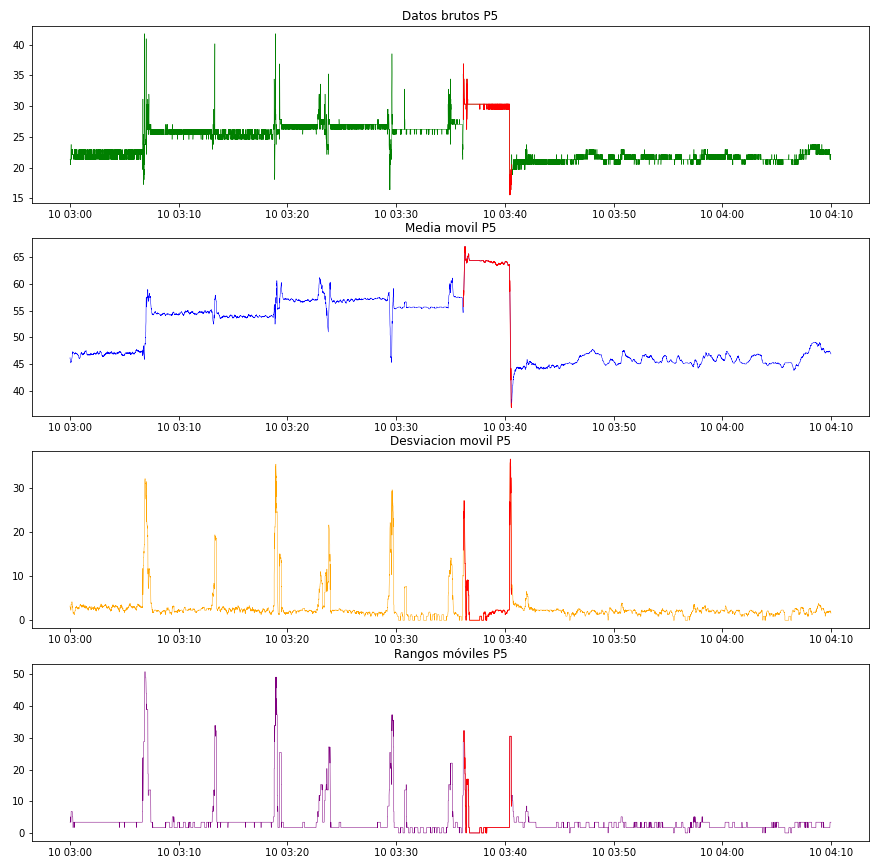
\includegraphics[width=1\textwidth]{images/SenalP5.png}
    \caption{Señales de los datos brutos y estadísticos asociados al tubo de presión P5. Crisis epiléptica en rojo.}
    \label{fig:senalP5}
\end{figure}

\chapter{Primeros pasos}
\section{Introducción}
En cuanto al trabajo hecho hasta el momento, vamos a hablar del preprocesado de los datos, incluyendo la carga de datos, la selección de los datos útiles y el cálculo estadísticas móviles (media y varianza). Hablamos también de las técnicas de reducción de dimensionalidad de los datos que hemos explorado, y cuáles hemos seleccionado, y algunas técnicas de filtrado. 

\section{Técnicas empleadas}
\begin{itemize}
\item Eliminación por baja señal y de datos erróneos
\item Eliminación manual de ruido
\item Normalización
\item Filtrados
\item Eliminación de baja variabilidad
\item Cálculo de estadísticas móviles 
\end{itemize}
\subsection{Eliminación por baja señal}
Nada más comenzar\footnote{Se aplica independientemente de que otras técnicas de procesamiento se empleen, la salida de esto se considera \textbf{bruta}}, y para todos los casos, hemos eliminado los datos que tienen por señal 0, (baja calidad) y todos los valores que no sean presiones también son eliminados debido a que en la mayor parte de las ocasiones dan valores no nulos de manera intermitente.

\subsection{Eliminación manual de ruido}
Observamos que en algunas ocasiones había datos aislados y valores muy pequeños o incluso negativos. Por ende, decidimos considerar todo valor menor de 5 como ruido y lo convertimos a 0. Con esta medida eliminamos también los valores negativos.
\subsection{Normalización}
Para trabajar siempre de la misma forma se normalizaron todos los datos, de 0 a 100, respecto a la presión
\subsection{Filtrados}
El filtrado es otra técnica empleada para eliminar el ruido, hemos empleado varias filtros como el \textit{butterworth}~\cite{wiki:butter} con valores \texttt{N=3} y \texttt{Wn=0.05} cuyo resultado se puede ver en la Figura~\ref{fig:senalP5butter}. Independientemente del tipo de filtro se aplican con la función \texttt{scipy.signal.filtfilt}. También se han probado el filtro \textit{Savitzky–Golay}~\cite{wiki:savgol} que se aplica con \texttt{scipy.signal.savgol\_filter} directamente el el resultado se puede ver en la Figura~\ref{fig:senalP5savgol}.
\begin{figure}
    \centering
    \begin{subfigure}[b]{\textwidth}
        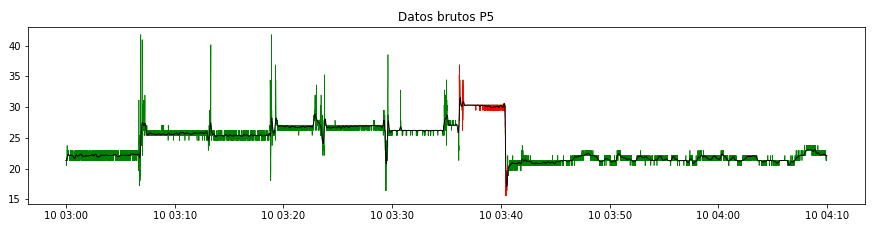
\includegraphics[width=1\textwidth]{images/SenalP5butter.png}
        \caption{Ejemplo de señal de presión filtrada mediante \textit{butterworth} con \texttt{N=3} y \texttt{Wn=0.05}. En verde la señal original y en negro la señal filtrada.}
        \label{fig:senalP5butter}
    \end{subfigure}
    \begin{subfigure}[b]{\textwidth}
        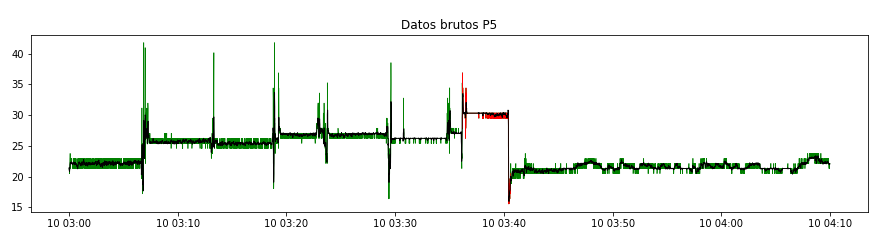
\includegraphics[width=1\textwidth]{images/SenalP5savgol.png}
        \caption{Ejemplo de señal de presión filtrada mediante \textit{Savitzky–Golay} con \texttt{window\_length=15} y \texttt{polyorder=2}. En verde la señal original y en negro la señal filtrada.}
        \label{fig:senalP5savgol}
    \end{subfigure}
    \caption{Filtrado de datos}
    \label{fig:filters}
\end{figure}

\subsection{Eliminación de baja variabilidad}
Para hacer más pequeño el conjunto de datos eliminamos aquellos tubos cuya variabilidad sea menor a un umbral, por defecto ese umbral de de 0.5.
\subsection{Cálculo de estadísticas móviles}
A partir de los datos calculamos la media móvil y la varianza móvil con una ventana de tamaño 25. El tamaño se ha escogido como aproximación inicial y se cambiará para futuras pruebas. 

\chapter{Transformadores}
\section{Introducción}
Hemos agrupado las distintas partes del preprocesado en \textit{Transformers} compatibles con sklearn~\cite{dreisbach_2015}. Los hemos dividido en varios grupos.
\section{Preprocesado}
Los transformadores de preprocesado son aquellos pensados para las operaciones básicas sobre los datos para facilitar la ejecución de otras más complejas. Las desarrolladas han sido:
\begin{itemize}
\item \texttt{Normalizer} para la normalización de los datos entre 0 y 1
\item \texttt{NoiseFilter(minimum=0)} transforma en 0 para valores menores del \texttt{minimum}
\item \texttt{VarianceThresholdPD(threshold=0.05)} elimina los datos con una varianza menor de \(0.05\) compatible con \texttt{pandas} al mantener los mismos nombres
\end{itemize}
\section{Estadísticos}
Para facilitar el procesado de estadísticos (media, desviación, rango, máximo y mínimo) hemos desarrollado un transformador genérico cuyos modos pueden ser \texttt{mean}, \texttt{std}, \texttt{range}, \texttt{max}, \texttt{min} y calcula una operación móvil sobre los datos. 

\texttt{StatisticsTransformer(mode='mean', window=25)}
\section{Filtrado}
Para el filtrado se han creado dos transformadores para dos filtros, \textit{ButterWorth} y \textit{Savitzky–Golay} aunque se pueden crear más extendiendo de \texttt{FilterTransformer()}. La signatura de los metodos sería:
\begin{itemize}
\item \texttt{ButterTransformer(N, Wn,btype='low', analog=False, output='ba', fs=None)}
\item \texttt{SavgolTransformer(window\_length, polyorder=2, deriv=0, delta=1.0, axis=-1, mode='interp', cval=0.0)}
\end{itemize}
\section{Compuestos}
Para agrupar distintos transformadores se han creado dos según la operación que se desea realizar, ya sea una concatenación (\texttt{ConcatenateTransformer}) y la aplicación en serie de transformadores (\texttt{PipelineTransformer}). Ambos reciben en sus constructores un conjunto indefinido de transformadores a aplicar en el orden deseado para aplicarlos.
\section{De instancias}
Los transformadores de instancias son aquellos que modifican completamente las instancias, incluyendo las fechas y las etiquetas. En particular el que existe en \texttt{MoveTargetsTransformer} que cambia los \textit{targets} de posición según una ventana para adaptar correctamente las ventanas según los valores de los estadísticos móviles.


Tiene cuatro modos, \texttt{only} que únicamente marca como crisis si el estadístico ha sido realizado solamente con datos de crisis, \texttt{half} donde se marca como crisis si al menos la mitad de los datos con los que se han realizado la estadística son crisis, \texttt{start} que marca como crisis si el primer elemento de los datos es una crisis y \texttt{end} que realiza lo contrario, si el último elemento es crisis\footnote{Los datos cuando son procesador con un estadístico cualquiera ya son de esta manera}
\chapter{Análisis de componentes principales (PCA)}
\section{Introducción}

Para comprobar si los datos de las presiones eran separables de manera fácil utilizamos PCA con los datos de las tres crisis documentadas a fecha de 2019-02-15.

\section{Preprocesamiento}
El preprocesamiento utilizado ha sido el filtro de ruido a 5, la normalización de los datos entre 0 y 100 y la eliminación de tubos con una varianza menor a 0.5. Además escogemos los datos que tengan un valor de SS mayor que 4000.

\section{Entrenamiento y testeo}
El análisis con la primera crisis Fig:~\ref{fig:pca_crisis1} tuvo de resultado que la crisis (rojo) no era separable de las situaciones normales (azul), además tampoco compartía espacio con las otras crisis (amarillo):

\begin{figure}
    \centering
    \begin{subfigure}[b]{0.45\textwidth}
        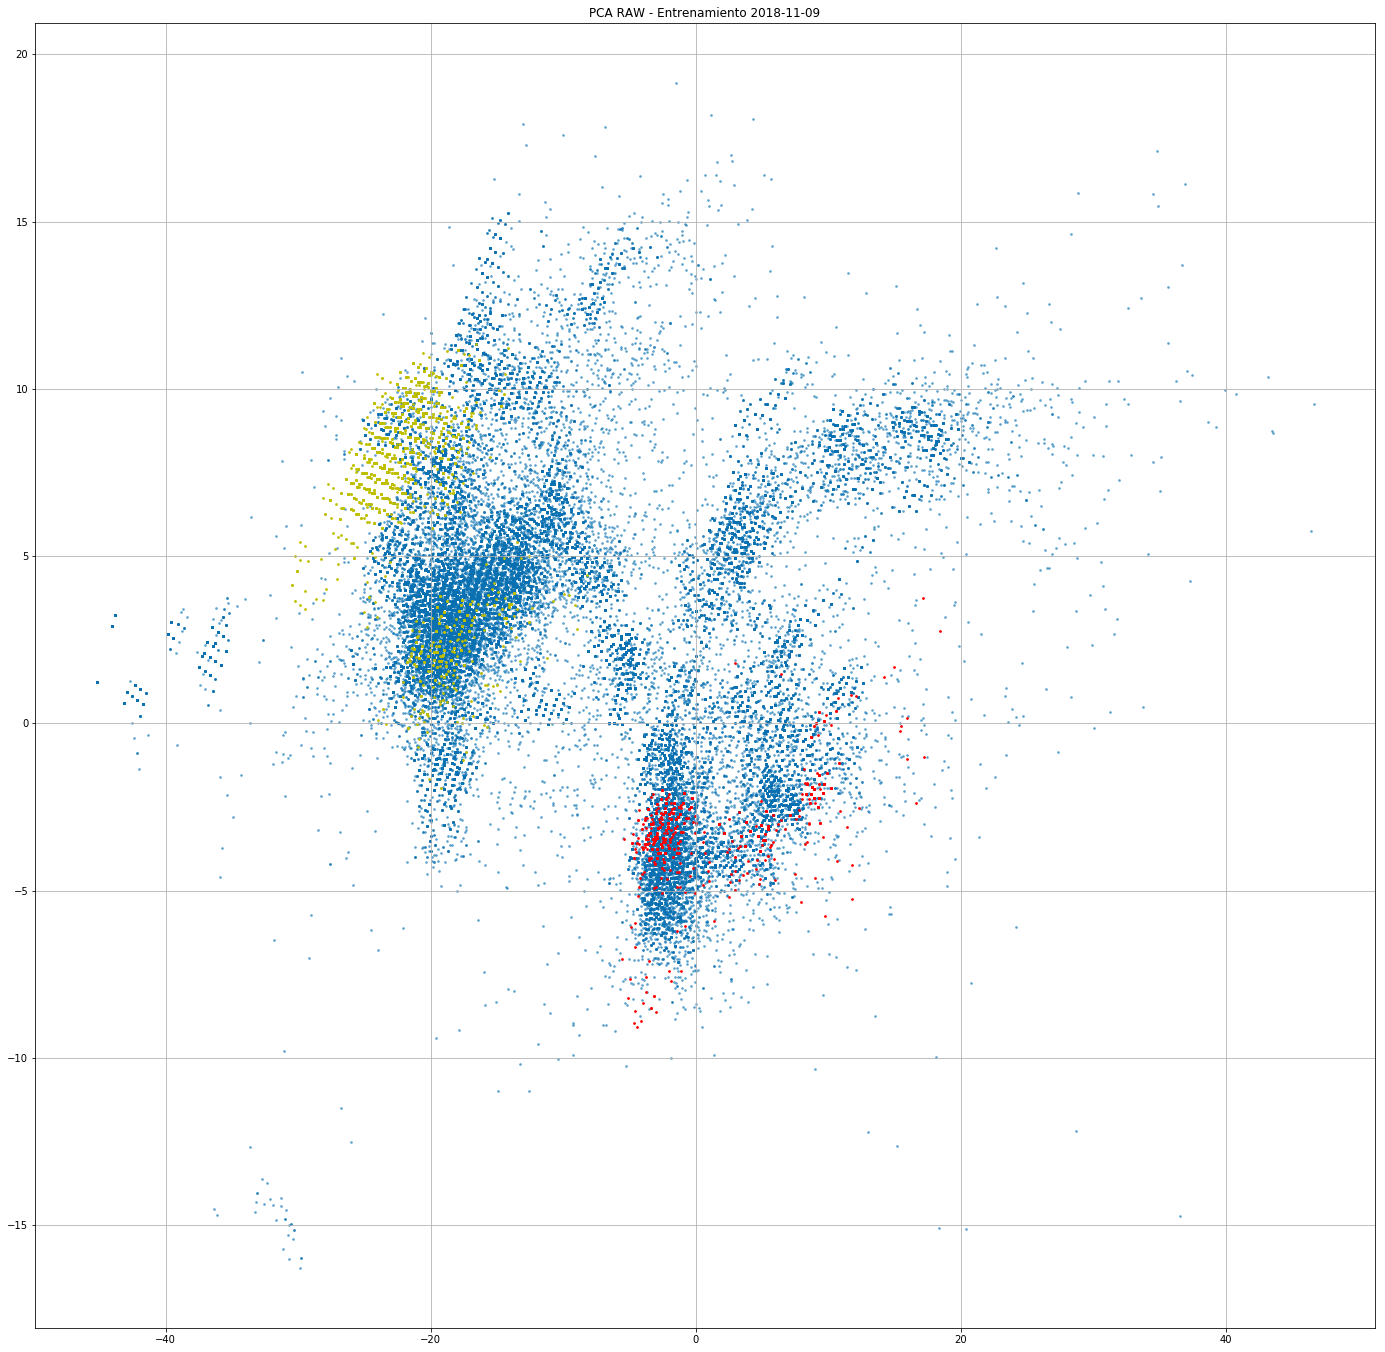
\includegraphics[width=\textwidth]{images/PCA-crisis1.png}
        \caption{Crisis 1}
        \label{fig:pca_crisis1}
    \end{subfigure}
    \begin{subfigure}[b]{0.45\textwidth}
        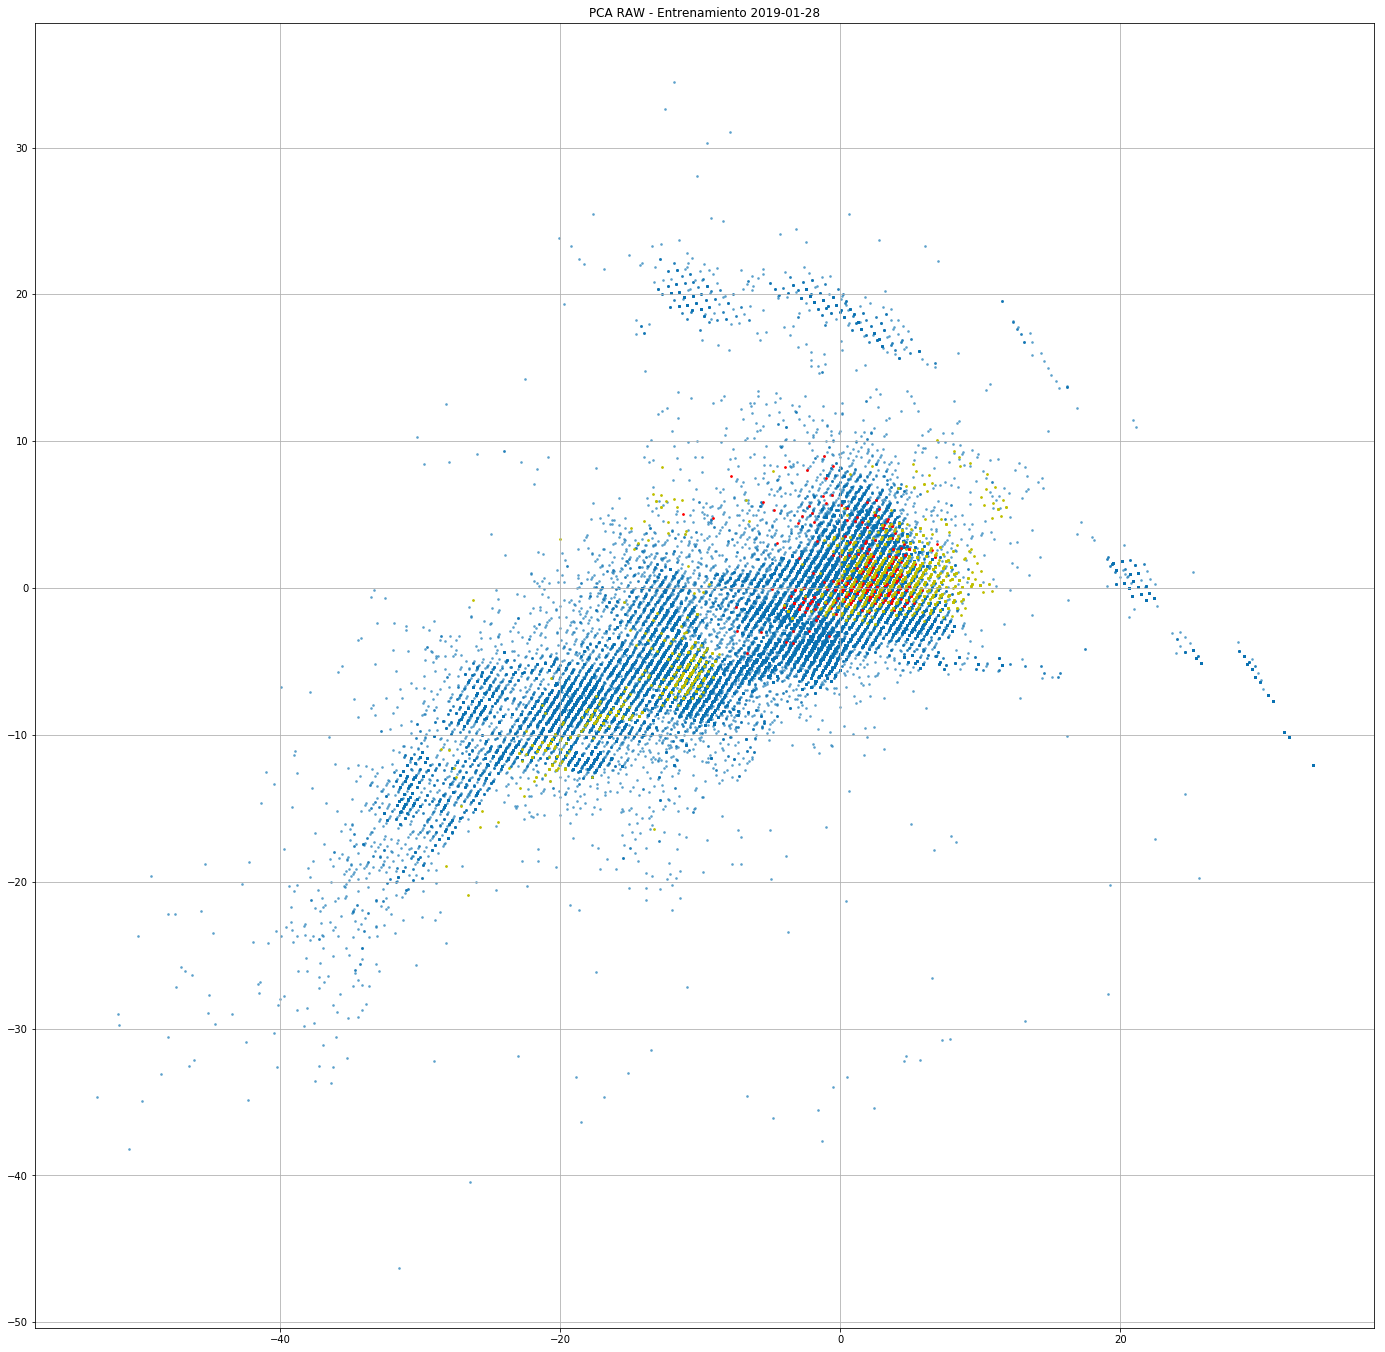
\includegraphics[width=\textwidth]{images/PCA-crisis2.png}
        \caption{Crisis 2}
        \label{fig:pca_crisis2}
    \end{subfigure}
    \begin{subfigure}[b]{0.45\textwidth}
        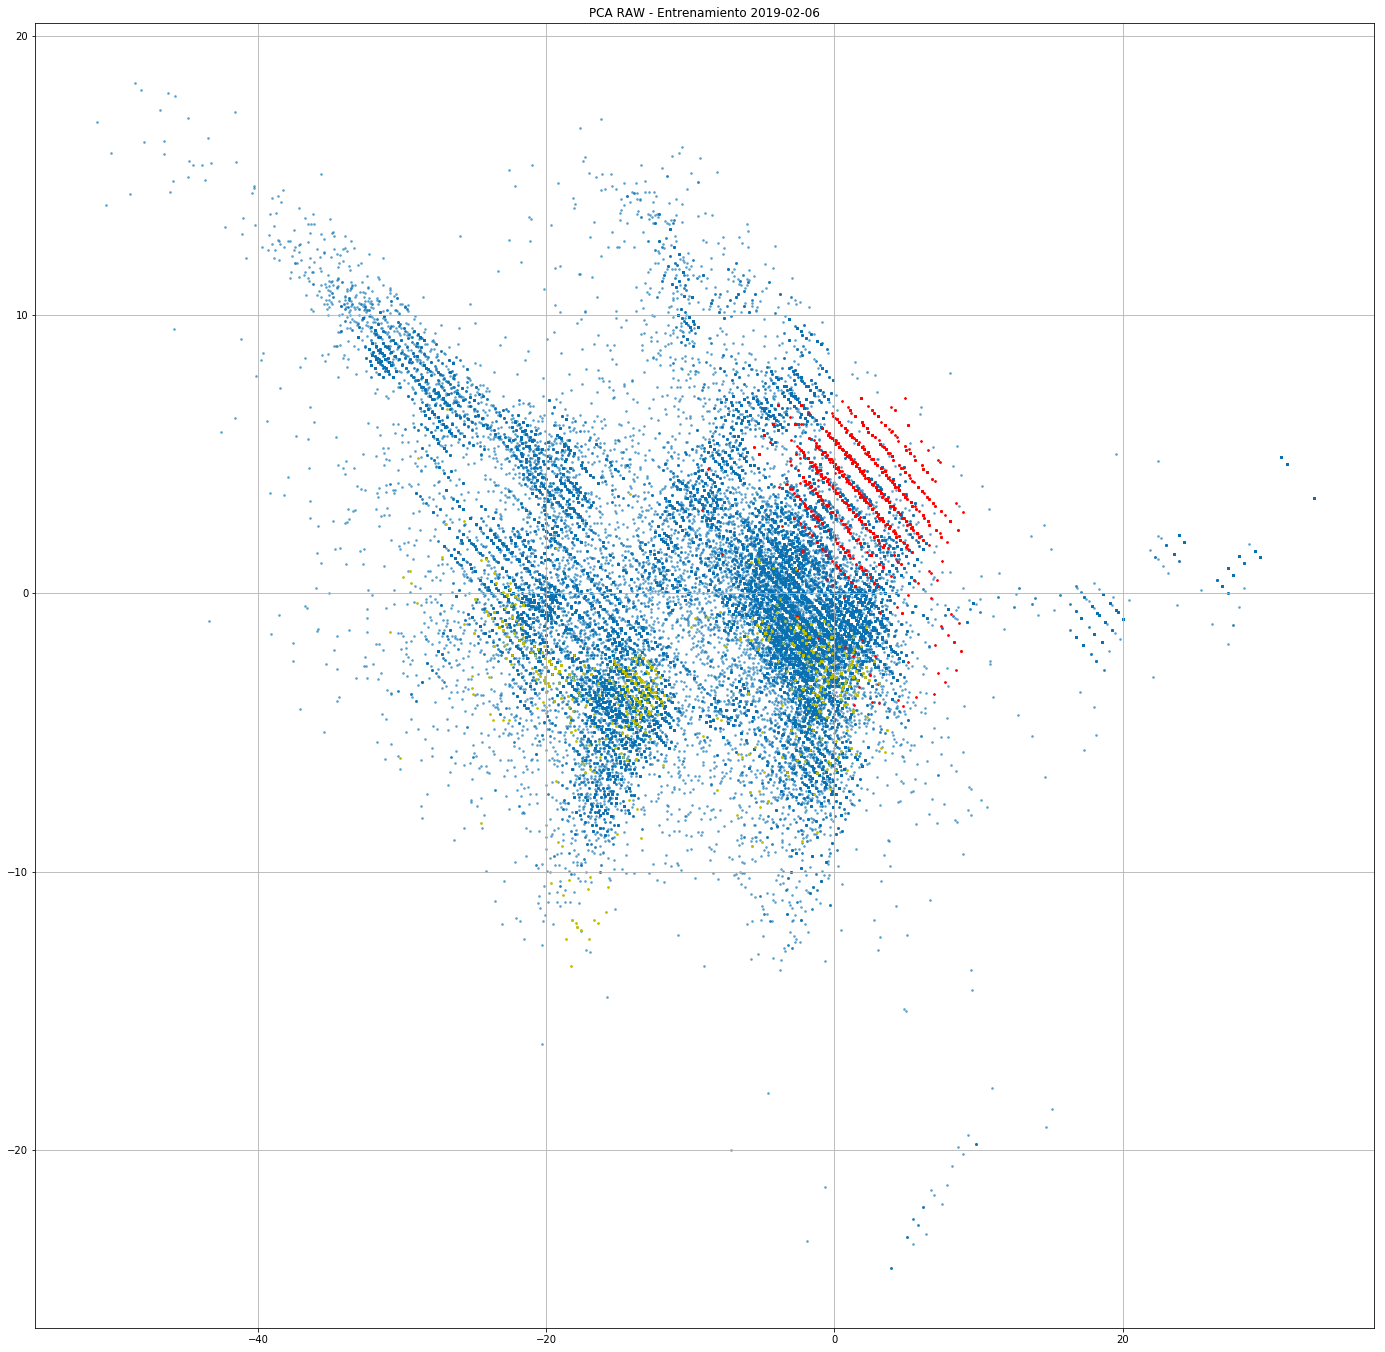
\includegraphics[width=\textwidth]{images/PCA-crisis3.png}
        \caption{Crisis 3}
        \label{fig:pca_crisis3}
    \end{subfigure}
    \caption{PCA ajustada a cada crisis}
\end{figure}

De manera semejante ocurre ajustando con la segunda crisis y la tercera Fig:~\ref{fig:pca_crisis2}, \ref{fig:pca_crisis3}

Si hacemos un ajuste con los datos de las tres crisis podemos ver que no son separables las situaciones de crisis y los datos normales Fig:~\ref{fig:pca_crisis_full}
\begin{figure}
    \centering
    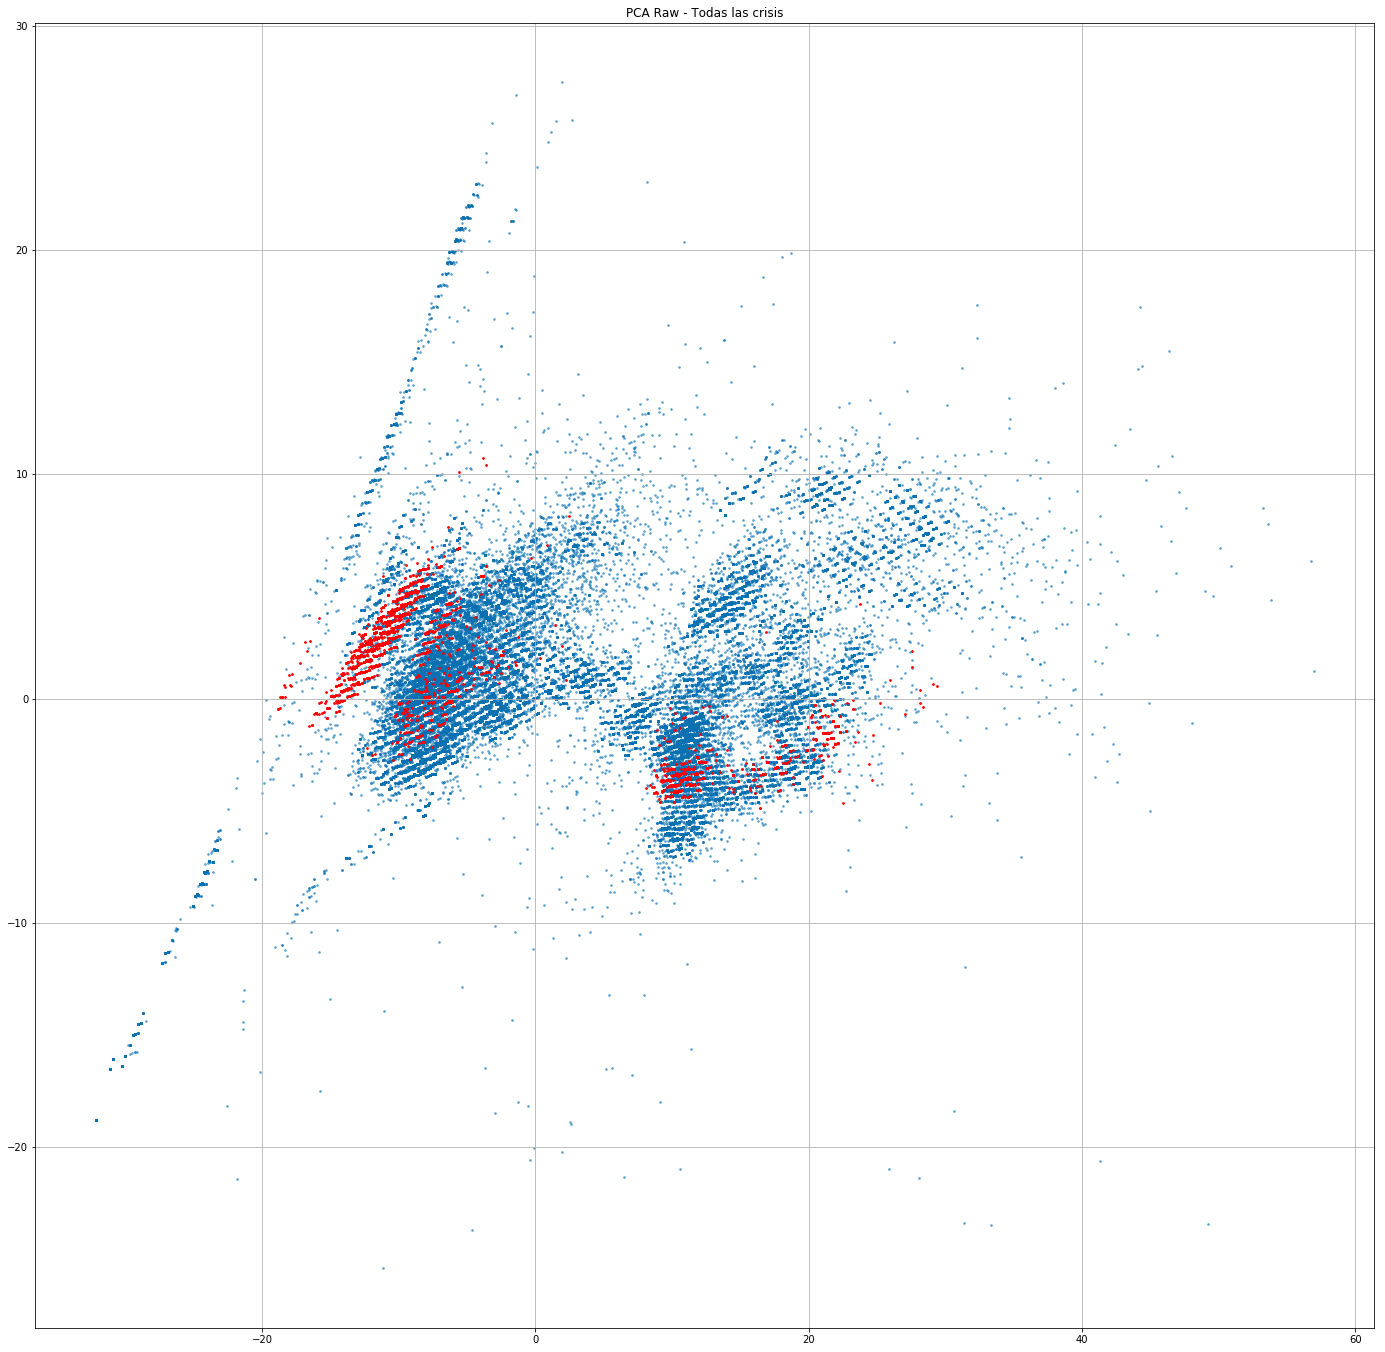
\includegraphics[width=\textwidth]{images/PCA-crisisFull.png}
    \caption{PCA ajustada con todas las crisis}
    \label{fig:pca_crisis_full}
\end{figure}
\chapter{Proyecciones a 2 dimensiones}
\section{Introducción}
También hemos aplicado las implementaciones de \texttt{sklearn.manifold} con los valores de presión correspondiente a la crisis que tuvo lugar el día 2018-11-10. El objetivo es comprobar si las crisis son fácilmente separables del resto de datos al realizar su proyección en un espacio de 2 dimensiones con alguna de las técnicas incluidas en la librería. A diferencia de PCA, estas implementaciones no permiten proyectar nuevos datos a partir de un modelo ya entrenado, por lo que la representación de las proyecciones solo incluirá los datos con los que se ha entrenado el modelo. Además, el volumen de datos que admiten estos métodos es limitado para los recursos que tenemos, lo que no nos permite entrenar los modelos con más de una crisis. Los parámetros de los métodos se han escogido teniendo en cuenta esta limitación. 
\section{Preprocesamiento}
Antes de aplicar las distintas técnicas se han realizado las siguientes operaciones: 
\begin{itemize}
    \item Selección de los datos comprendidos entre 20 minutos antes del inicio de la crisis y 20 minutos después de su finalización. 
    \item Filtro de ruido a 5 y normalización de los datos brutos entre 0 y 100.
    \item Cálculo de media, desviación y rangos móviles con ventana 25. 
    \item Normalización de los datos de media, desviación, y rango por separado para aplicar las proyecciones sobre ellos conjuntamente. 
    \item Filtro butterworth \texttt{N=3} y \texttt{Wn=0.05} tanto a los datos brutos como a los datos estadísticos.  
\end{itemize}

\section{Isomap}
Aplicamos Isomap~\cite{tenenbaum2000global} con \texttt{n\_neighbors=10} y \texttt{n\_components=2} a los datos en bruto (ver Fig:~\ref{fig:isomapDB}) y a los datos estadísticos (ver Fig:~\ref{fig:isomapDE}). 
\begin{figure}
    \centering
    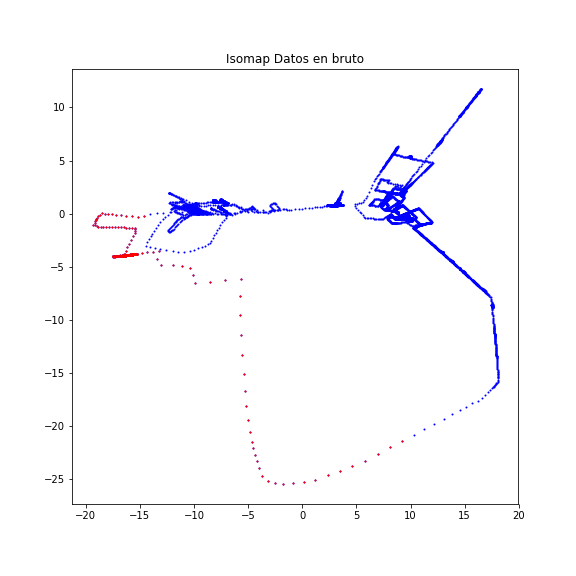
\includegraphics[width=0.75\textwidth]{images/isomapDB.png}
    \caption{Proyección Isomap 2D de los datos brutos de presiones. Crisis epiléptica en rojo.}
    \label{fig:isomapDB}
\end{figure}
\begin{figure}
    \centering
    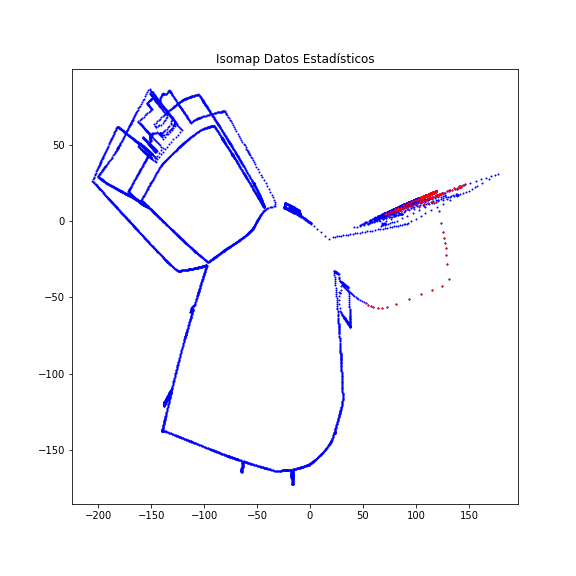
\includegraphics[width=0.75\textwidth]{images/isomapDE.png}
    \caption{Proyección Isomap 2D de los datos estadísticos de presiones. Crisis epiléptica en rojo.}
    \label{fig:isomapDE}
\end{figure}

\section{Locally Linear Embedding (LLE)}
Aplicamos LLE~\cite{roweis2000nonlinear} con \texttt{n\_neighbors=10} y \texttt{n\_components=2} a los datos en bruto (ver Fig:~\ref{fig:lleDB}) y a los datos estadísticos (ver Fig:~\ref{fig:lleDE}).
\begin{figure}
    \centering
    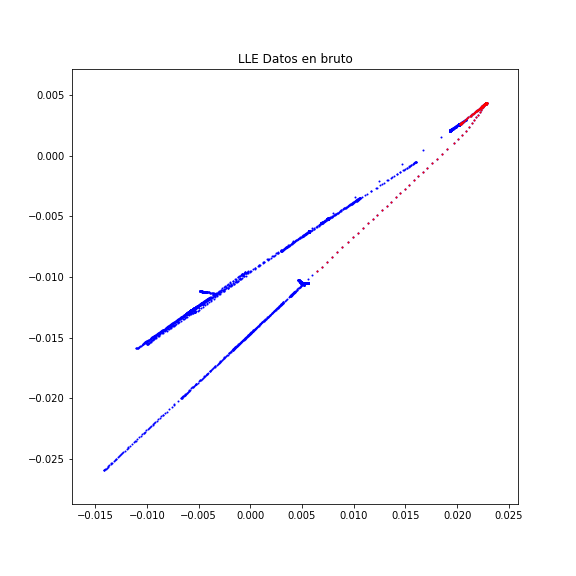
\includegraphics[width=0.75\textwidth]{images/lleDB.png}
    \caption{Proyección LLE 2D de los datos brutos de presiones. Crisis epiléptica en rojo.}
    \label{fig:lleDB}
\end{figure}
\begin{figure}
    \centering
    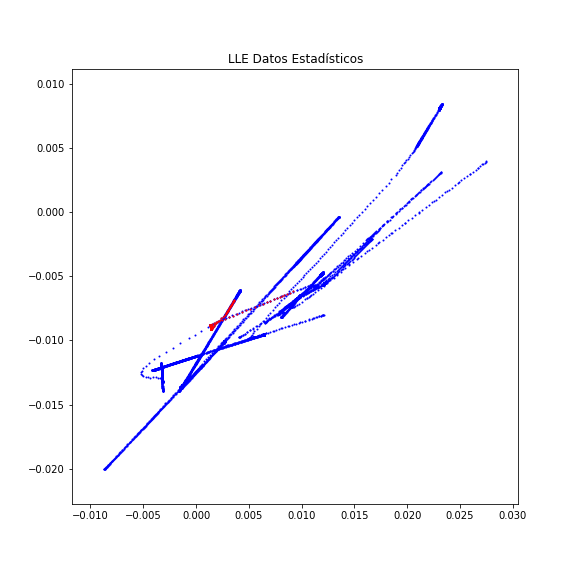
\includegraphics[width=0.75\textwidth]{images/lleDE.png}
    \caption{Proyección LLE 2D de los datos estadísticos de presiones. Crisis epiléptica en rojo.}
    \label{fig:lleDE}
\end{figure}
\section{Multi-dimensional Scaling (MDS)}
Aplicamos MDS~\cite{kruskal1964nonmetric,borg2003modern} con \texttt{n\_components=2} y \texttt{max\_iter=100} a los datos en bruto (ver Fig:~\ref{fig:mdsDB}) y a los datos estadísticos (ver Fig:~\ref{fig:mdsDE}).
\begin{figure}
    \centering
    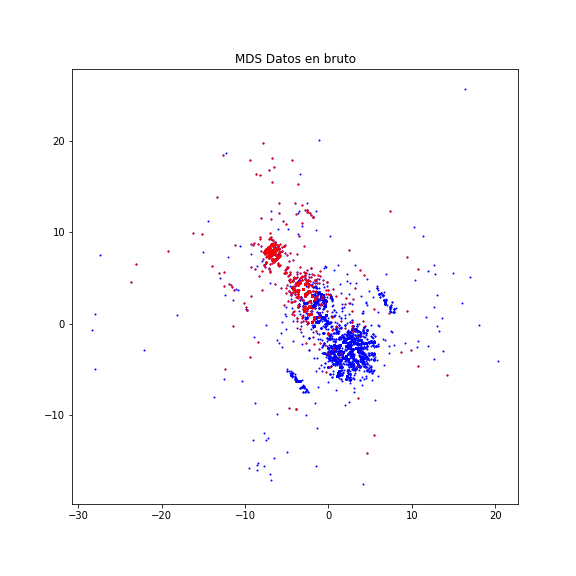
\includegraphics[width=0.75\textwidth]{images/mdsDB.png}
    \caption{Proyección MDS 2D de los datos brutos de presiones. Crisis epiléptica en rojo.}
    \label{fig:mdsDB}
\end{figure}
\begin{figure}
    \centering
    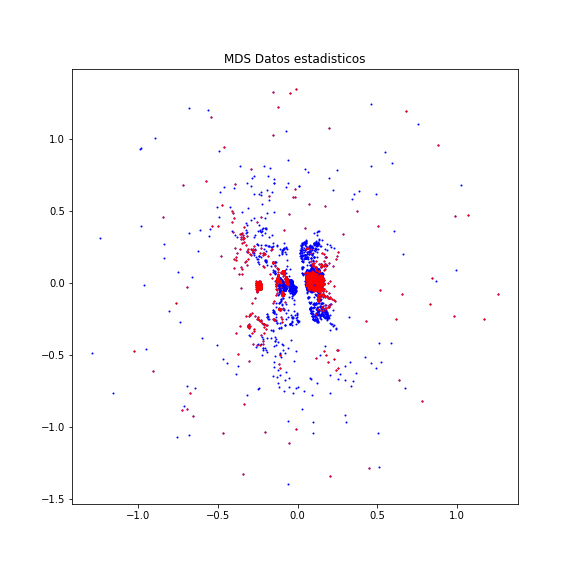
\includegraphics[width=0.75\textwidth]{images/mdsDE.png}
    \caption{Proyección MDS 2D de los datos estadísticos de presiones. Crisis epiléptica en rojo.}
    \label{fig:mdsDE}
\end{figure}
\section{Otros métodos}
Se han empleado otros métodos cuyas proyecciones no merecen ser consideradas al no presentar ningún tipo de separación aparente entre los datos de la crisis y el resto. 
\begin{itemize}
    \item Modified Locally Linear Embedding (MLLE~\cite{zhang2007mlle}) con \texttt{n\_neighbors=15} y \texttt{n\_components=2}.
    \item Hessian Eigenmapping con \texttt{n\_neighbors=20} y \texttt{n\_components=2}. 
\end{itemize}
\chapter{One-Class simple}
\section{Introducción}
Debido a que el problema que intentamos resolver es desequilibrado~\cite{galar2012review} una línea que hemos explorado ha sido la detección de anomalías, por tanto se ha probado a entrenar un clasificador de \textit{One-Class} de máquina de vectores soporte (SVM) con sklearn.
\section{Configuración}
La configuración del clasificador ha sido la por defecto teniendo en cuenta un \textit{kernel} de tipo \textit{Radial Basis Function}~\cite{wiki:rbf}, \texttt{gamma} de \(0.01\) y \texttt{nu} de \(0.1\) 
\section{Preprocesado}
Se han probado seis configuraciones de preprocesado distintas, tres bases y las equivalentes en estadísticas móviles, estas han sido de ventana 25. A su vez, cada estadística por separado (Media, desviación y rango) ha sido normalizado entre 0 y 100. Además se han eliminado aquellas columnas con una varianza menor a 0.5.\footnote{Aunque esto no ha perturbado los datos}
Los procesados han sido dos más los valores en bruto\footnote{Eliminado ruido en el umbral \(5\), normalizado entre 0 y 100 y eliminación de tubos con poca varianza menor de 0.5}. Se han aplicado el filtro \texttt{scipy.signal.savgol\_filter} con ventana de \(15\) y, paralelamente, un filtro \texttt{scipy.signal.butter} con los valores \(3\) y \(0.05\)

\section{Entrenamiento}
El entrenamiento se ha realizado de manera alternativa entre solo crisis o la situación normal con todos los conjuntos de datos puestos con anterioridad. En particular se han usado los datos de la noche entre el 9 y el 10 de noviembre de 2018 que contiene una crisis documentada entre las 03:30:00 y las 3:50:00. Aunque se consideró el inicio real como 03:36:10 porque los valores cambian abruptamente y las 03:40:37 cuando vuelven a cambiar abruptamente. 

También probamos a entrenar con la primera y la segunda crisis. Esta que fue el 28 de enero la consideramos entre las 2019-01-29 06:12:04 y las 2019-01-29 06:15:37 al ser el área más anómala de la crisis debido a que la crisis no estaba etiquetada correctamente.

La tercera crisis, fue el 6 de febrero y esta fue etiquetada correctamente.\footnote{Aunque en precisión de minutos y no de segundos.}

\section{Resultados}
Los resultados entrenando con el conjunto de no crisis fueron en una matriz de confusión no diagonalmente dominante, por tanto solamente nos centraremos en la predicción con el entrenamiento de no crisis
\subsection{Datos de entrenamiento}
El entrenamiento se realizó de dos maneras distintas, una utilizando solamente datos de la primera crisis y otra utilizando los datos de las dos primeras crisis. Los resultados se pueden ver en las tablas agrupadas en la Tabla~\ref{tab:matriz-conf-1a} para el entrenamiento con una crisis y Tabla~\ref{tab:matriz-conf-1a-2d} con las dos primeras crisis
\begin{table}
    \begin{center}
        %RAW
        \begin{subtable}[c]{0.4\textwidth}
            \begin{tabular}{lrc}
                \hline
                 & No Crisis & Crisis \\
                \hline
                No Crisis & 103419 & 6 \\
                Crisis & 71 & 553\\
                \hline
            \end{tabular}
            \subcaption{Datos Brutos}
            \label{tab:mat-conf-raw-1.1}
        \end{subtable}
        \hspace{1em}\vspace{1em}
        \begin{subtable}[c]{0.4\textwidth}
                \begin{tabular}{lrc}
                \hline
                 & No Crisis & Crisis \\
                \hline
                No Crisis & 103426 & 0 \\
                Crisis & 59 & 540\\
                \hline
            \end{tabular}
            \subcaption{Datos Estadísticos}
            \label{tab:mat-conf-stats-1.1}
        \end{subtable}
        %SavGol
        
        \begin{subtable}[c]{0.4\textwidth}
            \begin{tabular}{lrc}
                \hline
                 & No Crisis & Crisis \\
                \hline
                No Crisis & 103421 & 4 \\
                Crisis & 62 & 562\\
                \hline
            \end{tabular}
            \subcaption{Filtrado Savitzky–Golay}
            \label{tab:mat-conf-raw-1.2}
        \end{subtable}
        \hspace{1em}\vspace{1em}
        \begin{subtable}[c]{0.4\textwidth}
                \begin{tabular}{lrc}
                \hline
                 & No Crisis & Crisis \\
                \hline
                No Crisis & 103426 & 0 \\
                Crisis & 60 & 539\\
                \hline
            \end{tabular}
            \subcaption{Savitzky–Golay Estadístico}
            \label{tab:mat-conf-stats-1.2}
        \end{subtable}
        %Butter
        
        \begin{subtable}[c]{0.4\textwidth}
            \begin{tabular}{lrc}
                \hline
                 & No Crisis & Crisis \\
                \hline
                No Crisis & 103425 & 0 \\
                Crisis & 62 & 562\\
                \hline
            \end{tabular}
            \subcaption{Filtrado ButterWorth}
            \label{tab:mat-conf-raw-1.3}
        \end{subtable}
        \hspace{1em}\vspace{1em}
        \begin{subtable}[c]{0.4\textwidth}
                \begin{tabular}{lrc}
                \hline
                 & No Crisis & Crisis \\
                \hline
                No Crisis & 103426 & 0 \\
                Crisis & 61 & 538\\
                \hline
            \end{tabular}
            \subcaption{ButterWorth Estadístico}
            \label{tab:mat-conf-stats-1.3}
        \end{subtable}
        \caption{Matrices de confusión entrenamiento con 1º crisis}
        \label{tab:matriz-conf-1a}
    \end{center}
\end{table}

\begin{table}
    \begin{center}
        %RAW
        \begin{subtable}[c]{0.4\textwidth}
            \begin{tabular}{lrc}
                \hline
                 & No Crisis & Crisis \\
                \hline
                No Crisis & 171109 & 36209 \\
                Crisis & 117 & 1042\\
                \hline
            \end{tabular}
            \subcaption{Datos Brutos}
            \label{tab:mat-conf-raw-1.4}
        \end{subtable}
        \hspace{1em}\vspace{1em}
        \begin{subtable}[c]{0.4\textwidth}
                \begin{tabular}{lrc}
                \hline
                 & No Crisis & Crisis \\
                \hline
                No Crisis & 207295 & 0 \\
                Crisis & 122 & 1012\\
                \hline
            \end{tabular}
            \subcaption{Datos Estadísticos}
            \label{tab:mat-conf-stats-1.4}
        \end{subtable}
        %SavGol
        
        \begin{subtable}[c]{0.4\textwidth}
            \begin{tabular}{lrc}
                \hline
                 & No Crisis & Crisis \\
                \hline
                No Crisis & 185987 & 21331 \\
                Crisis & 116 & 1043\\
                \hline
            \end{tabular}
            \subcaption{Filtrado Savitzky–Golay}
            \label{tab:mat-conf-raw-1}
        \end{subtable}
        \hspace{1em}\vspace{1em}
        \begin{subtable}[c]{0.4\textwidth}
                \begin{tabular}{lrc}
                \hline
                 & No Crisis & Crisis \\
                \hline
                No Crisis & 207295 & 0 \\
                Crisis & 122 & 1012\\
                \hline
            \end{tabular}
            \subcaption{Savitzky–Golay Estadístico}
            \label{tab:mat-conf-stats-1.5}
        \end{subtable}
        %Butter
        
        \begin{subtable}[c]{0.4\textwidth}
            \begin{tabular}{lrc}
                \hline
                 & No Crisis & Crisis \\
                \hline
                No Crisis & 192713 & 14605 \\
                Crisis & 115 & 1044\\
                \hline
            \end{tabular}
            \subcaption{Filtrado ButterWorth}
            \label{tab:mat-conf-raw-1.6}
        \end{subtable}
        \hspace{1em}\vspace{1em}
        \begin{subtable}[c]{0.4\textwidth}
                \begin{tabular}{lrc}
                \hline
                 & No Crisis & Crisis \\
                \hline
                No Crisis & 207295 & 0 \\
                Crisis & 164 & 970\\
                \hline
            \end{tabular}
            \subcaption{ButterWorth Estadístico}
            \label{tab:mat-conf-stats-1.6}
        \end{subtable}
        \caption{Matrices de confusión entrenamiento con 1º y 2º crisis}
        \label{tab:matriz-conf-1a-2d}
    \end{center}
\end{table}


\subsection{Datos de test}
La validación se ha realizado con la segunda y tercera crisis (por separado) para el entrenamiento con una sola crisis y la tercera crisis cuando se ha entrenado con las dos primeras. Los resultados se pueden ver en Tabla~\ref{tab:matriz-test-2a} y Tabla~\ref{tab:matriz-test-3a} para las validaciones con el entrenamiento de una sola crisis y en Tabla~\ref{tab:matriz-test-2-3a} para las validaciones con el entrenamiento de las dos primeras crisis.
\begin{table}
    \begin{center}
        %RAW
        \begin{subtable}[c]{0.4\textwidth}
            \begin{tabular}{lrc}
                \hline
                 & No Crisis & Crisis \\
                \hline
                No Crisis & 103893 & 0 \\
                Crisis & 535 & 0\\
                \hline
            \end{tabular}
            \subcaption{Datos Brutos}
            \label{tab:mat-conf-raw-test-1.7}
        \end{subtable}
        \hspace{1em}\vspace{1em}
        \begin{subtable}[c]{0.4\textwidth}
                \begin{tabular}{lrc}
                \hline
                 & No Crisis & Crisis \\
                \hline
                No Crisis & 103894 & 0 \\
                Crisis & 510 & 0\\
                \hline
            \end{tabular}
            \subcaption{Datos Estadísticos}
            \label{tab:mat-conf-stats-test-1.7}
        \end{subtable}
        %SavGol
        \begin{subtable}[c]{0.4\textwidth}
            \begin{tabular}{lrc}
                \hline
                 & No Crisis & Crisis \\
                \hline
                No Crisis & 103893 & 0 \\
                Crisis & 535 & 0\\
                \hline
            \end{tabular}
            \subcaption{Filtrado Savitzky–Golay}
            \label{tab:mat-conf-raw-test-1.8}
        \end{subtable}
        \hspace{1em}\vspace{1em}
        \begin{subtable}[c]{0.4\textwidth}
                \begin{tabular}{lrc}
                \hline
                 & No Crisis & Crisis \\
                \hline
                No Crisis & 103894 & 0 \\
                Crisis & 510 & 0\\
                \hline
            \end{tabular}
            \subcaption{Savitzky–Golay Estadístico}
            \label{tab:mat-conf-stats-1.7}
        \end{subtable}
        %Butter
        \begin{subtable}[c]{0.4\textwidth}
            \begin{tabular}{lrc}
                \hline
                 & No Crisis & Crisis \\
                \hline
                No Crisis & 103893 & 0 \\
                Crisis & 535 & 0\\
                \hline
            \end{tabular}
            \subcaption{Filtrado ButterWorth}
            \label{tab:mat-conf-raw-1.7}
        \end{subtable}
        \hspace{1em}\vspace{1em}
        \begin{subtable}[c]{0.4\textwidth}
                \begin{tabular}{lrc}
                \hline
                 & No Crisis & Crisis \\
                \hline
                No Crisis & 103894 & 0 \\
                Crisis & 510 & 0\\
                \hline
            \end{tabular}
            \subcaption{ButterWorth Estadístico}
            \label{tab:mat-conf-stats-1.8}
        \end{subtable}
        \caption{Matriz de confusión test con 2º crisis (entrenamiento con 1ª)}
        \label{tab:matriz-test-2a}
    \end{center}
\end{table}

\begin{table}
    \begin{center}
        %RAW
        \begin{subtable}[c]{0.4\textwidth}
            \begin{tabular}{lrc}
                \hline
                 & No Crisis & Crisis \\
                \hline
                No Crisis & 86990 & 0 \\
                Crisis & 2741 & 0\\
                \hline
            \end{tabular}
            \subcaption{Datos Brutos}
            \label{tab:mat-conf-raw-1.8}
        \end{subtable}
        \hspace{1em}\vspace{1em}
        \begin{subtable}[c]{0.4\textwidth}
                \begin{tabular}{lrc}
                \hline
                 & No Crisis & Crisis \\
                \hline
                No Crisis & 86975 & 0 \\
                Crisis & 2732 & 0\\
                \hline
            \end{tabular}
            \subcaption{Datos Estadísticos}
            \label{tab:mat-conf-stats-1.9}
        \end{subtable}
        %SavGol
        \begin{subtable}[c]{0.4\textwidth}
            \begin{tabular}{lrc}
                \hline
                 & No Crisis & Crisis \\
                \hline
                No Crisis & 86990 & 0 \\
                Crisis & 2741 & 0\\
                \hline
            \end{tabular}
            \subcaption{Filtrado Savitzky–Golay}
            \label{tab:mat-conf-raw-1.9}
        \end{subtable}
        \hspace{1em}\vspace{1em}
        \begin{subtable}[c]{0.4\textwidth}
                \begin{tabular}{lrc}
                \hline
                 & No Crisis & Crisis \\
                \hline
                No Crisis & 86975 & 0 \\
                Crisis & 2732 & 0\\
                \hline
            \end{tabular}
            \subcaption{Savitzky–Golay Estadístico}
            \label{tab:mat-conf-stats-1.10}
        \end{subtable}
        %Butter
        \begin{subtable}[c]{0.4\textwidth}
            \begin{tabular}{lrc}
                \hline
                 & No Crisis & Crisis \\
                \hline
                No Crisis & 86990 & 0 \\
                Crisis & 2741 & 0\\
                \hline
            \end{tabular}
            \subcaption{Filtrado ButterWorth}
            \label{tab:mat-conf-raw-1.10}
        \end{subtable}
        \hspace{1em}\vspace{1em}
        \begin{subtable}[c]{0.4\textwidth}
                \begin{tabular}{lrc}
                \hline
                 & No Crisis & Crisis \\
                \hline
                No Crisis & 86975 & 0 \\
                Crisis & 2732 & 0\\
                \hline
            \end{tabular}
            \subcaption{ButterWorth Estadístico}
            \label{tab:mat-conf-stats-1.11}
        \end{subtable}
        \caption{Matriz de confusión test 3º crisis (entrenamiento 1º)}
        \label{tab:matriz-test-3a}
    \end{center}
\end{table}

\begin{table}
    \begin{center}
        %RAW
        \begin{subtable}[c]{0.4\textwidth}
            \begin{tabular}{lrc}
                \hline
                 & No Crisis & Crisis \\
                \hline
                No Crisis & 86713 & 277 \\
                Crisis & 2741 & 0\\
                \hline
            \end{tabular}
            \subcaption{Datos Brutos}
            \label{tab:mat-conf-raw-1.11}
        \end{subtable}
        \hspace{1em}\vspace{1em}
        \begin{subtable}[c]{0.4\textwidth}
                \begin{tabular}{lrc}
                \hline
                 & No Crisis & Crisis \\
                \hline
                No Crisis & 86975 & 0 \\
                Crisis & 2732 & 0\\
                \hline
            \end{tabular}
            \subcaption{Datos Estadísticos}
            \label{tab:mat-conf-stats-1.12}
        \end{subtable}
        %SavGol
        \begin{subtable}[c]{0.4\textwidth}
            \begin{tabular}{lrc}
                \hline
                 & No Crisis & Crisis \\
                \hline
                No Crisis & 86898 & 92 \\
                Crisis & 2741 & 0\\
                \hline
            \end{tabular}
            \subcaption{Filtrado Savitzky–Golay}
            \label{tab:mat-conf-raw-1.12}
        \end{subtable}
        \hspace{1em}\vspace{1em}
        \begin{subtable}[c]{0.4\textwidth}
                \begin{tabular}{lrc}
                \hline
                 & No Crisis & Crisis \\
                \hline
                No Crisis & 86975 & 0 \\
                Crisis & 2732 & 0\\
                \hline
            \end{tabular}
            \subcaption{Savitzky–Golay Estadístico}
            \label{tab:mat-conf-stats-1.13}
        \end{subtable}
        %Butter
        \begin{subtable}[c]{0.4\textwidth}
            \begin{tabular}{lrc}
                \hline
                 & No Crisis & Crisis \\
                \hline
                No Crisis & 86967 & 23 \\
                Crisis & 2741 & 0\\
                \hline
            \end{tabular}
            \subcaption{Filtrado ButterWorth}
            \label{tab:mat-conf-raw-1.13}
        \end{subtable}
        \hspace{1em}\vspace{1em}
        \begin{subtable}[c]{0.4\textwidth}
                \begin{tabular}{lrc}
                \hline
                 & No Crisis & Crisis \\
                \hline
                No Crisis & 86975 & 0 \\
                Crisis & 2732 & 0\\
                \hline
            \end{tabular}
            \subcaption{ButterWorth Estadístico}
            \label{tab:mat-conf-stats-1.14}
        \end{subtable}
        \caption{Matriz de confusión test 3º crisis (entrenamiento con 1º y 2º)}
        \label{tab:matriz-test-2-3a}
    \end{center}
\end{table}


Como se puede observar los resultados de los test son muy negativos por lo que se ha desechado esta línea de investigación

\chapter{\textit{Ensembles} para desequilibrados}\label{chap:ensdes}
\section{Introducción}
Otra línea de investigación ha sido la utilización de \textit{ensembles} optimizados para aprendizaje desequilibrado, seguimos dos líneas al utilizar algunos de los algoritmos presentados en la revisión de Galar~et.~al.~\cite{galar2012review} y los resultados de Diez~et.~al.~\cite{diez2015diversity}. En particular utilizamos en primera instancia el filtro SMOTE~\cite{wiki:smote} aplicado a \textit{Bagging} y \textit{AdaBoostM1} y \textit{RotationForest}~\cite{rodriguez2006rotation}.

Los test fueron realizados con \textit{Weka}~\textit{3.7} y se entrenó con las medias y varianzas móviles de tamaño noventa con las dos primeras crisis, con un SMOTE con un porcentaje de $1000\%$ y testeado con la tercera crisis con el mismo preprocesado.

\section{Resultados}
\subsection{Train-Test}
Se puede observar en la Tabla~\ref{tab:matriz-smote-2-3a} que siempre tenemos un acierto nulo al testear los datos. Es destacable observar que incluso en el caso de \textit{AdaBoost} (Tabla~\ref{tab:mat-conf-ada-train}) el entrenamiento falla por lo que podemos deducir que los datos no están bien etiquetados ya que este algoritmo se centra en los datos que falla en predecir y en situaciones de ruido tiene un desempeño peor. Esta prueba además de la etiquetación poco precisa de las crisis existentes nos hace pensar que el sistema realmente es muy ruidoso.
\begin{table}
    \begin{center}
        %Bagging
        \begin{subtable}[c]{0.4\textwidth}
            \begin{tabular}{lrc}
                \hline
                 & No Crisis & Crisis \\
                \hline
                No Crisis & 203274   & 0 \\
                Crisis & 1 & 55274  \\
                \hline
            \end{tabular}
            \subcaption{Bagging - Train}
            \label{tab:mat-conf-bagg-train}
        \end{subtable}
        \hspace{1em}\vspace{1em}
        \begin{subtable}[c]{0.4\textwidth}
            \begin{tabular}{lrc}
                \hline
                 & No Crisis & Crisis \\
                \hline
                No Crisis & 86936 & 0 \\
                Crisis & 2706 & 0\\
                \hline
            \end{tabular}
            \subcaption{Bagging - Test}
            \label{tab:mat-conf-bagg-test}
        \end{subtable}
        %AdaBoost
        \begin{subtable}[c]{0.4\textwidth}
            \begin{tabular}{lrc}
                \hline
                 & No Crisis & Crisis \\
                \hline
                No Crisis & 203274 & 0 \\
                Crisis & 55275 & 0\\
                \hline
            \end{tabular}
            \subcaption{AdaBoostM1 - Train}
            \label{tab:mat-conf-ada-train}
        \end{subtable}
        \hspace{1em}\vspace{1em}
        \begin{subtable}[c]{0.4\textwidth}
            \begin{tabular}{lrc}
                \hline
                 & No Crisis & Crisis \\
                \hline
                No Crisis & 86936 & 0 \\
                Crisis & 2706 & 0\\
                \hline
            \end{tabular}
            \subcaption{AdaBoostM1 - Test}
            \label{tab:mat-conf-ada-test}
        \end{subtable}
        %Rotation Forest
        \begin{subtable}[c]{0.4\textwidth}
            \begin{tabular}{lrc}
                \hline
                 & No Crisis & Crisis \\
                \hline
                No Crisis & 203274  & 0 \\
                Crisis & 1 & 55274\\
                \hline
            \end{tabular}
            \subcaption{Rotation Forest - Train}
            \label{tab:mat-conf-rotfor-train}
        \end{subtable}
        \hspace{1em}\vspace{1em}
        \begin{subtable}[c]{0.4\textwidth}
            \begin{tabular}{lrc}
                \hline
                 & No Crisis & Crisis \\
                \hline
                No Crisis &  86936 & 0 \\
                Crisis & 2706 & 0\\
                \hline
            \end{tabular}
            \subcaption{Rotation Forest - Test}
            \label{tab:mat-conf-rotfor-test}
        \end{subtable}
    \caption{Matrices de confusión - SMOTE Train-Test}
    \label{tab:matriz-smote-2-3a}
    \end{center}
\end{table}
\begin{table}
    \begin{center}
        %Dos primeras
        \begin{subtable}[c]{0.4\textwidth}
            \begin{tabular}{lrc}
                \hline
                 & No Crisis & Crisis \\
                \hline
                No Crisis & 203274  & 0 \\
                Crisis & 2 & 5023 \\
                \hline
            \end{tabular}
            \subcaption{Fold 1-Dos primeras crisis}
            \label{tab:mat-conf-rotfor-two-fold1}
        \end{subtable}
        \hspace{1em}\vspace{1em}
        \begin{subtable}[c]{0.4\textwidth}
            \begin{tabular}{lrc}
                \hline
                 & No Crisis & Crisis \\
                \hline
                No Crisis & 203274  & 0 \\
                Crisis & 9 & 5016\\
                \hline
            \end{tabular}
            \subcaption{Fold 2-Dos primeras crisis}
            \label{tab:mat-conf-rotfor-two-fold2}
        \end{subtable}
        %Todas
        \begin{subtable}[c]{0.4\textwidth}
            \begin{tabular}{lrc}
                \hline
                 & No Crisis & Crisis \\
                \hline
                No Crisis & 290210  & 0 \\
                Crisis & 1 & 7730\\
                \hline
            \end{tabular}
            \subcaption{Fold 1 - Todas las crisis}
            \label{tab:mat-conf-rotfor-all-fold1}
        \end{subtable}
        \hspace{1em}\vspace{1em}
        \begin{subtable}[c]{0.4\textwidth}
            \begin{tabular}{lrc}
                \hline
                 & No Crisis & Crisis \\
                \hline
                No Crisis & 290209 & 1 \\
                Crisis & 16 & 7715\\
                \hline
            \end{tabular}
            \subcaption{Fold 2 - Todas las crisis}
            \label{tab:mat-conf-rotfor-all-fold2}
        \end{subtable}
    \caption{Matrices de confusión - SMOTE CrossValidation}
    \label{tab:matriz-smote-cv}
    \end{center}
\end{table}

\subsection{Validación cruzada}
Además de estos experimentos realizamos una validación cruzada con dos subconjuntos de las dos primeras crisis y todas las crisis con el mismo prepocesamiento. Usamos \textit{RotationForest} ya que es el que mejor desempeño demostró en el caso anterior. El desempeño se puede ver en la Tabla~\ref{tab:matriz-smote-cv} y aunque el resultado es muy bueno, a la hora de testear el modelo entrenado con las dos primeras crisis con la tercera no se clasifica ningún valor como crisis.

\section{Conclusiones}
De estas pruebas se deducen diferentes conclusiones, primero que los datos que tenemos no están bien etiquetados y son ruidosos y que las diferencias entre las distintas crisis son muy amplias dando a entender que posiblemente no se trata de un sobreajuste sino que los datos entre las distintas crisis está muy separado como pudimos ver en PCA.


\chapter{Random Forest -- Media y desviación móviles} 
\section{Introducción}
En este apartado hemos tratado de encontrar la mejor configuración posible de valores para las ventanas a las que se aplican la media y la desviación de las presiones, con el objetivo de comprobar si es posible entrenar un buen clasificador usando únicamente estas características en lugar de otras más elaboradas y difíciles de calcular. El objetivo era encontrar el mejor área bajo la curva ROC~\cite{galar2012review}, la cual representa el ratio de verdaderos positivos frente a los falsos positivos. Sin embargo, esta métrica puede presentar una visión demasiado optimista del rendimiento del algoritmo cuando se trabaja en el contexto de un conjunto de datos muy desequilibrado~\cite{Davis2006RPR, saito2015pr}, como es nuestro caso. Por ello y adicionalmente, realizaremos las mismas operaciones teniendo en consideración una métrica más adecuada para conjuntos desequilibrados, la curva Precision-Recall. 

\section{Modificación del target}
Al trabajar con datos calculados a partir de una ventana, hay que tener en cuenta que existen varias formas de considerar como ``crisis'' una instancia de dato calculada de esta forma. Nosotros definimos 3 formas distintas: 

\begin{itemize}
    \item Labeled if all are crisis: Etiquetamos como ``crisis'' la instancia si todos los datos de presión que se han usado para calcularla estaban etiquetados como ``crisis''. 
    \item Labeled if half are crisis: Etiquetamos como ``crisis'' la instancia si al menos la última mitad de los datos de presión que se han usado para calcularla estaban etiquetados como ``crisis''. 
    \item Labeled if one is crisis: Etiquetamos como ``crisis'' la instancia si el último dato de presión usado para calcularla estaba etiquetado como ``crisis''. 
\end{itemize}

\section{Validación cruzada entre dos días}\label{rf1}

Para todos los modelos del clasificador Random Forest considerados en los siguientes apartados se empleará el mismo procedimiento de testeo para calcular su rendimiento. Se usarán los datos de 2 días distintos en los que existe una crisis epiléptica y se seguirán los siguientes pasos: 

\begin{enumerate}
    \item Se entrenará el clasificador con los datos del día de la primera crisis y testeado con los de la segunda. 
    \item Se calculará el rendimiento de acuerdo a la métrica correspondiente (ROC o Precision-Recall según el caso) con los resultados del testeo (auc1\footnote{AUC del testeo entrenando con la primera crisis}). 
    \item Se entrenará el clasificador con los datos del día de la segunda crisis y testeado con los de la primera. 
    \item Se calculará el rendimiento con los resultados del testeo (auc2\footnote{AUC del testeo entrenando con la segunda crisis}). 
    \item Se calculará el rendimiento final como la media entre auc1 y auc2. Buscamos que el rendimiento final sea lo mayor posible. 
\end{enumerate}

\section{Primera exploración, métrica=ROC}

Hemos realizado una primera exploración combinando de todas las formas posibles las siguientes ventanas y estrategias de modificación del target: 
\begin{itemize}
    \item Ventanas para la media = [5, 30, 55, 80, 105, 130, 155, 180]
    \item Ventanas para la desviación = [5, 30, 55, 80, 105, 130, 155, 180]
    \item Modificación del target = [`Labeled if all are crisis', `Labeled if half are crisis', `Labeled if one is crisis']
\end{itemize}
 
Por cada combinación de ventana para la media, ventana para la desviación, y estrategia de modificación del target se han aplicado ambos cálculos estadísticos a las presiones de 2 días distintos en los que existe una crisis epiléptica y se han usado esos datos estadísticos para llevar a cabo el proceso de validación definido en el apartado anterior.

Tras realizar todas las ejecuciones, la mejor área bajo la curva (ROC = 0.72) se ha encontrado con la siguiente combinación: 
\begin{itemize}
    \item Ventana para la media = 105
    \item Ventana para la desviación = 80
    \item Modificación del target = 'Labeled if all are crisis'
\end{itemize}

En las figuras~\ref{fig:heatmap1}, \ref{fig:heatmap2} y \ref{fig:heatmap3} el eje vertical representa la ventana para la desviación y el eje horizontal la ventana para la media. 

\begin{figure}
    \centering
    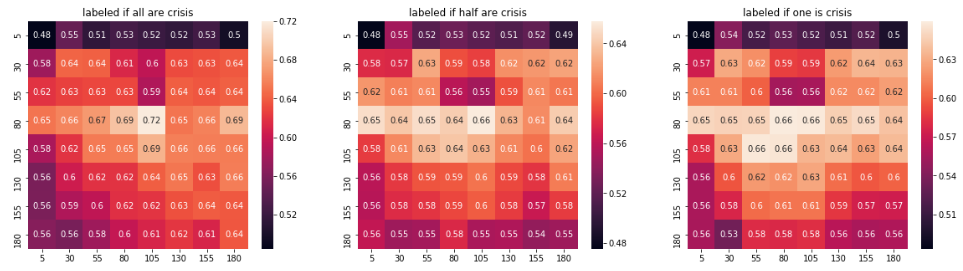
\includegraphics[width=1\textwidth]{images/heatmap1.png}
    \caption{Mapa de calor de las áreas bajo la curva calculadas en la primera exploración con la métrica=ROC.}
    \label{fig:heatmap1}
\end{figure}

\section{Segunda exploración, métrica=ROC}

A continuación, centramos la exploración en ventanas cercanas a las que han ofrecido mejores resultados en la exploración anterior, teniendo en cuenta que, como se aprecia en la figura Fig:~\ref{fig:heatmap1}, el resultado parece ser más dependiente de la ventana de la desviación que la de la media: 
\begin{itemize}
    \item Ventanas para la media = [5, 30, 55, 80, 105, 130, 155, 180]
    \item Ventanas para la desviación = [70, 75, 80, 85, 90, 95, 100, 105, 110]
    \item Modificación del target = ['Labeled if all are crisis', 'Labeled if half are crisis', 'Labeled if one is crisis']
\end{itemize}

Realizando las mismas operaciones, la mejor área bajo la curva (roc = 0.76) se ha encontrado con la siguiente combinación: 
\begin{itemize}
    \item Ventana para la media = 105
    \item Ventana para la desviación = 75
    \item Modificación del target = 'Labeled if all are crisis'
\end{itemize}

\begin{figure}
    \centering
    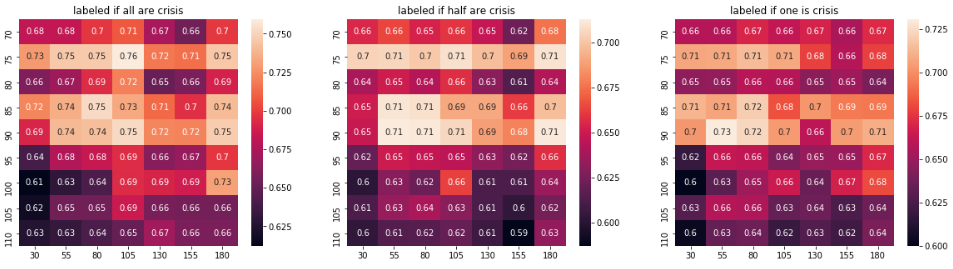
\includegraphics[width=1\textwidth]{images/heatmap2.png}
    \caption{Mapa de calor de las áreas bajo la curva calculadas en la segunda exploración con la métrica=ROC.}
    \label{fig:heatmap2}
\end{figure}

\section{Tercera exploración, métrica=ROC}
Finalmente, centramos la exploración un poco más: 
\begin{itemize}
    \item Ventanas para la media = [40, 65, 90, 115, 140, 165, 190]
    \item Ventanas para la desviación = [80, 82, 84, 86, 88, 90, 92, 94]
    \item Modificación del target = ['Labeled if all are crisis', 'Labeled if half are crisis', 'Labeled if one is crisis']
\end{itemize}

La mejor área bajo la curva (roc=0.76) se ha encontrado con la siguiente combinación: 
\begin{itemize}
    \item Ventana para la media = 90
    \item Ventana para la desviación = 90
    \item Modificación del target = 'Labeled if all are crisis'
\end{itemize}

\begin{figure}
    \centering
    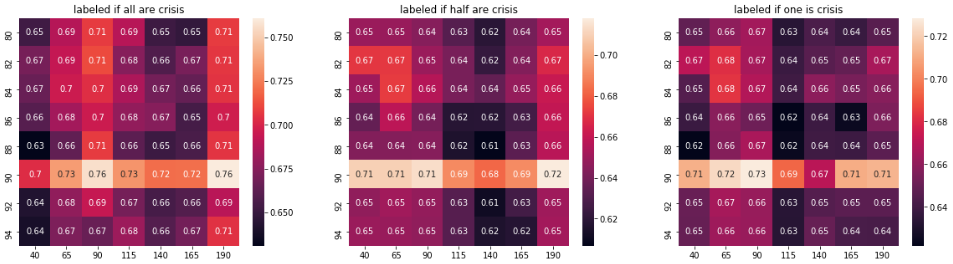
\includegraphics[width=1\textwidth]{images/heatmap3.png}
    \caption{Mapa de calor de las áreas bajo la curva calculadas en la tercera exploración con la métrica=ROC.}
    \label{fig:heatmap3}
\end{figure}

\section{Primera exploración, métrica=Precision-Recall}

Al igual que con la otra métrica, hemos realizado una primera exploración combinando de todas las formas posibles las siguientes ventanas y estrategias de modificación del target: 
\begin{itemize}
    \item Ventanas para la media = [5, 30, 55, 80, 105, 130, 155, 180]
    \item Ventanas para la desviación = [5, 30, 55, 80, 105, 130, 155, 180]
    \item Modificación del target = ['Labeled if all are crisis', 'Labeled if half are crisis', 'Labeled if one is crisis']
\end{itemize}

Tras la validación de todas las ejecuciones, la mejor precisión media (average\_precision\_score = 0.026) se ha encontrado con la siguiente combinación: 
\begin{itemize}
    \item Ventana para la media = 55
    \item Ventana para la desviación = 105
    \item Modificación del target = 'Labeled if one are crisis'
\end{itemize}

\begin{figure}
    \centering
    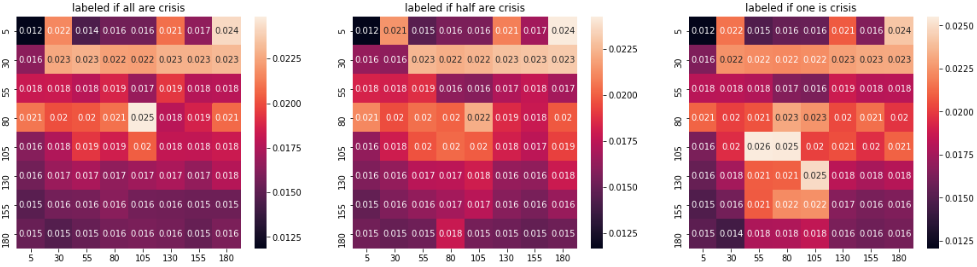
\includegraphics[width=1\textwidth]{images/heatmap4.png}
    \caption{Mapa de calor de las áreas bajo la curva calculadas en la primera exploración con la métrica=Precision-Recall.}
    \label{fig:heatmap4}
\end{figure}

\section{Segunda exploración, métrica=Precision-Recall}

A continuación, centramos la exploración en ventanas cercanas a las que han ofrecido mejores resultados en la exploración anterior:

\begin{itemize}
    \item Ventanas para la media = [40, 65, 90, 115, 140, 165, 190]
    \item Ventanas para la desviación = [70, 75, 80, 85, 90, 95, 100]
    \item Modificación del target = ['Labeled if all are crisis', 'Labeled if half are crisis', 'Labeled if one is crisis']
\end{itemize}

Realizando las mismas operaciones, la mejor precisión media(average\_precision\_score = 0.035) se ha encontrado con la siguiente combinación: 
\begin{itemize}
    \item Ventana para la media = 65
    \item Ventana para la desviación = 85
    \item Modificación del target = 'Labeled if one are crisis'
\end{itemize}

\begin{figure}
    \centering
    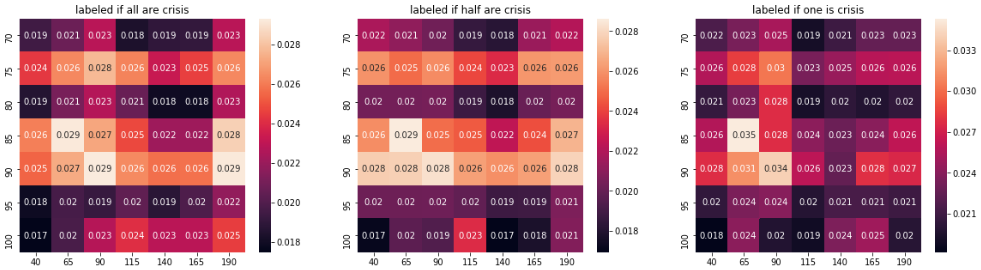
\includegraphics[width=1\textwidth]{images/heatmap5.png}
    \caption{Mapa de calor de las áreas bajo la curva calculadas en la segunda exploración con la métrica=Precision-Recall.}
    \label{fig:heatmap5}
\end{figure}

\section{Tercera exploración, métrica=Precision-Recall}
Finalmente, centramos la exploración un poco más: 
\begin{itemize}
    \item Ventanas para la media = [40, 65, 90, 115, 140, 165, 190]
    \item Ventanas para la desviación = [80, 82, 84, 86, 88, 90, 92, 94]
    \item Modificación del target = ['Labeled if all are crisis', 'Labeled if half are crisis', 'Labeled if one is crisis']
\end{itemize}

La mejor precisión media (average\_precision\_score=0.034) se ha encontrado con la siguiente combinación: 
\begin{itemize}
    \item Ventana para la media = 90
    \item Ventana para la desviación = 90
    \item Modificación del target = 'Labeled if one are crisis'
\end{itemize}

\begin{figure}
    \centering
    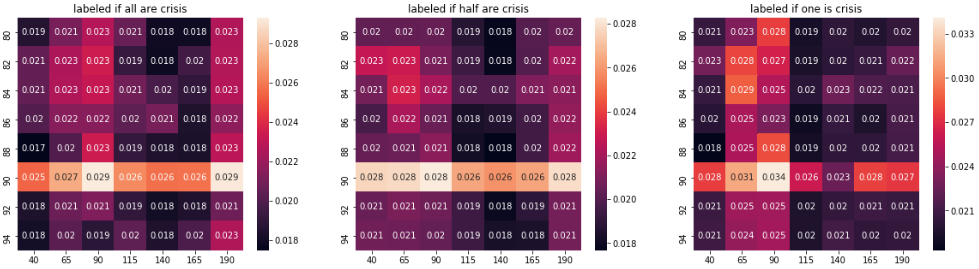
\includegraphics[width=1\textwidth]{images/heatmap6.png}
    \caption{Mapa de calor de las áreas bajo la curva calculadas en la tercera exploración con la métrica=Precision-Recall.}
    \label{fig:heatmap6}
\end{figure}

Observamos que al igual que con la otra métrica, el valor óptimo de las ventanas resulta ser el mismo, por lo que para cualquier cálculo posterior se empleará un tamaño de ventana de 90 instancias. 

\chapter{Extracción de características con \textit{tsfresh} y clasificador Random Forest}
\section{Introducción}
Como alternativa a estadísticas más simples como la media y la desviación, hemos utilizado la librería tsfresh~\cite{christ2018time} para extracción de características en series temporales. Dado que en las exploraciones anteriores, obtenemos los mejores resultados con una ventana de 90 tanto para la media como para la desviación, asumimos este valor de ventana para el cálculo de estas características. Utilizando la función \texttt{tsfresh.extract\_features} con los parámetros por defecto obtenemos 794 características por cada columna. Si lo aplicamos a las columnas relativas a cada uno de los 6 tubos de presión obtenemos un total de 4764 características, demasiadas para entrenar el clasificador, por lo que planteamos varias formas de filtrar las más útiles. 

\section{Filtrado típico de características}

A partir de las características obtenidas en el apartado anterior, nuestra primera aproximación es filtrar aplicando una serie de operaciones generales de filtrado una tras otra para ir reduciendo la cantidad de características. Realizamos las siguientes operaciones en este orden: 
\begin{enumerate}
    \item Eliminar las características (columnas) con algún valor nulo, ya que provocará fallos en pasos posteriores. 
    \item Eliminar las características con formatos no admitidos por los pasos posteriores. En nuestro caso los siguientes filtros fallan al aplicarlos a la característica \texttt{\_\_sample\_\_entropy}, por lo que la eliminamos. 
    \item Eliminar las características con baja varianza usando \texttt{sklearn.feature\_selection.VarianceThreshold} con un threshold de 0.01. 
    \item Seleccionar las 1000 mejores características usando \texttt{sklearn.feature\_selection.SelectKBest} con \texttt{score\_func=sklearn.feature\_selection.chi2} (función chi cuadrado). 
    \item Seleccionamos las mejores características en función a un modelo. En nuestro caso hemos usado un modelo de clasificación Random Forest con valor de threshold=0.02 (teniendo en cuenta que los valores están normalizados entre 0 y 1). Este filtrado es supervisado ya que también recibe los valores de target. 
\end{enumerate}
Una vez realizados estos pasos nos quedan 7 características. Con estas 7 realizamos la misma operación descrita en el apartado \ref{rf1} (entrenando con los datos de un día y testeando con los de otro, y viceversa) para cada una de las métricas de rendimiento: 

\begin{itemize}
    \item Para la métrica ROC obtenemos un área bajo la curva final de 0.61. 
    \item Para la métrica Precision-Recall obtenemos una precisión media de 0.022.
\end{itemize}

Ambas mediciones del rendimiento resultan muy lejos de lo deseable. Con distintas variaciones de los parámetros de las operaciones utilizadas obtenemos resultados similares.

\section{Filtrado mediante la función \texttt{select\_features} de tsfresh}
Dados los malos resultados obtenidos mediante el filtrado del apartado anterior, de forma alternativa hemos probado a usar la función
\texttt{tsfresh.feature\_selection.selection.select\_features} para la selección de atributos. Esta selección también es supervisada ya que recibe los targets junto con las características a filtrar. Tras aplicar esta función seguimos teniendo 1731 características, por lo que planteamos una estrategia adicional para eliminar las menos relevantes. Si asumimos que una característica será relevante si resulta relevante para todos los datos sobre los que se ha calculado, nos quedaremos solo con aquellas características que tras el filtrado, permanezcan para los 6 tubos de presión iniciales. De esta forma nos quedamos únicamente con 744 características (124 por cada tubo de presión). 

\section{Selección del mejor conjunto de características}

Tras realizar el paso anterior obtenemos 124 características distintas aplicadas a cada uno de los 6 tubos de presión que podemos emplear para entrenar un clasificador RandomForest. Al mantener las 6 columnas asociadas a cada característica, podemos entrenarlo usando solo una característica (6 columnas de datos) o un conjunto mayor de ellas. Para escoger qué subconjunto de características mínimo nos permite obtener mejores resultados hemos planteado dos estrategias: 

\begin{itemize}
    \item Aplicar el clasificador RandomForest a cada una y realizar un ranking inicial sobre el que trabajar. 
    \item Emplear un algoritmo genético
\end{itemize}

\subsection{Ranking en función de la métrica de evaluación}
Esta estrategia consiste en aplicar el clasificador RandomForest a cada característica por separado (6 columnas de datos) de la misma forma que en los aparatos anteriores (validación cruzada entre 2 días), y obtener el rendimiento (ya sea mediante ROC o mediante Precision-Recall). Para cada métrica generamos un ranking, el cual sitúa más arriba a aquellas características que hayan obtenido un rendimiento mayor. 

\begin{itemize}
    \item La mejor característica usando la ROC como métrica (\texttt{\_\_change\_quantiles(qh=1.0,ql=0.4)}) obtiene un área bajo la curva de 0.8. 
    \item La mejor característica usando Precision-Recall como métrica (\texttt{\_\_change\_quantiles(qh=1.0,ql=0.4)}) obtiene un rendimiento medio de 0.099. 
\end{itemize}

A partir de cada uno de los rankings podemos hacer combinaciones de varias formas: 

\begin{itemize}
    \item En primer lugar probamos a ir añadiendo características en el orden en el que se sitúan en el ranking para el entrenamiento del clasificador. Probaremos con las características 1 y 2, las 1, 2 y 3, las 1, 2, 3 y 4\dots y así sucesivamente hasta que el área bajo la curva obtenida deje de aumentar. 
    \begin{itemize}
        \item Usando la ROC como métrica comprobamos que la combinación de las características 1 y 2 ya ofrece un área bajo la curva peor, de 0.78, por lo que parece probable que combinar características buenas no produce necesariamente mejores resultados.
        \item Usando Precision-Recall como métrica obtenemos que la combinación de las características 1 y 2.
        \\(\texttt{\_\_change\_quantiles(f\_agg="mean", isabs=True,\\ qh=1.0, ql=0.4)} y \texttt{\_\_number\_peaks(n=1)}) ofrece un rendimiento medio algo mejor, de 0.107. Sin embargo la combinación 1, 2 y 3 ya ofrece peores resultados.
    \end{itemize} 
    \item En segundo lugar probamos a combinar la mejor característica con todas las demás y comprobar si el área bajo la curva aumenta. Probamos así con las características 1 y 2, las 1 y 3, las 1 y 4\dots y así sucesivamente. 
    \begin{itemize}
        \item Usando la ROC, en este caso comprobamos que el área bajo la curva mejora con dos de las combinaciones. Con las combinaciones de las características 1 y 3 (\texttt{\_\_change\_quantiles(f\_agg="mean", isabs=True, qh=1.0, ql=0.4)} y \texttt{\_\_change\_quantiles(\\f\_agg="var", isabs=False, qh=1.0, ql=0.4)}), y las características 1 y 5 (\texttt{\_\_change\_quantiles(f\_agg="mean", isabs=True, qh=1.0,\\ ql=0.4)} y \texttt{\_\_symmetry\_looking(r=0.25)}) se obtiene un área bajo la curva de 0.83. 
        \item Usando Precision-Recall encontramos 32 combinaciones que mejoran la precisión media, siendo la combinación de las características 1 y 11 (\texttt{\_\_change\_quantiles(f\_agg="mean", isabs=True, qh=1.0, ql=0.4)} y \texttt{\_\_change\_quantiles(f\_agg="var",\\ isabs=True, qh=0.8, ql=0.4)}) la que ofrece un mejor resultado, de 0.142. 
    \end{itemize}
\end{itemize}

\subsection{Algoritmo genético}
Como alternativa a los métodos planteados en el apartado anterior probamos un algoritmo genético para la selección de la mejor combinación de características. Para ello vamos a usar la librería  deap~\cite{DEAP_JMLR2012}, un framework de python para computación evolutiva. 


\begin{itemize}
    \item \textbf{Genotipo:} A partir del ranking de características calculado en el apartado anterior, planteamos un genotipo en el que cada individuo puede incluir una combinación de como máximo 10 características. Para ello usamos un array de tamaño 10 que contiene números enteros. Cada gen (número entero) identifica una de las características del ranking (realizaremos una ejecución para cada uno de los 2 rankings, es decir, para cada una de las métricas planteadas). 
    \item \textbf{Fenotipo:} La evaluación de cada individuo consistirá en entrenar y testear mediante validación cruzada de 2 días el clasificador Random Forest, usando las características indicadas por los genes del individuo concreto. El valor de fitness del individuo corresponderá con el valor final del rendimiento (calculado dependiendo de la métrica escogida) calculado por este método. Dado que utilizamos un método de cruce no adecuado para permutaciones, es posible que en el genotipo aparezcan genes repetidos. En este caso a la hora de evaluar solo se añadirá esa característica una vez, haciendo que el conjunto final de características pueda ser menor de 10. 
    \item \textbf{Método de cruce:} Cruce uniforme con probabilidad de 0.5 por cada gen. 
    \item \textbf{Método de mutación:} Mutación por modificación de gen por otro permitido con una probabilidad de 0.2 por gen.
    \item \textbf{Método de selección: } Selección por torneo con tamaño 3. 
    \item \textbf{Probabilidad de cruce:} Se aplicará la operación de cruce sobre un individuo de la población con una probabilidad de 0.6. 
    \item \textbf{Probabilidad de mutación:} Se aplicará la operación de mutación sobre un individuo de la población con una probabilidad de 0.1. 
    \item \textbf{Tamaño de la población: } 50 individuos. 
    \item \textbf{Número de generaciones: } 50. El número de generaciones se ha escogido teniendo en cuenta lo costoso que es el procedimiento de evaluación de cada individuo, pero consideramos que ha resultado ser suficiente ya que no se ha producido ninguna mejora en las últimas 18 generaciones. 
\end{itemize}

\subsubsection{Resultados usando la ROC como métrica:} 

Tras la evolución el mayor valor de área bajo la curva que se ha logrado es de 0.8587 con las características indicadas por el individuo [28, 54, 23, 68, 83, 97, 61, 120, 44, 64]. Es el mayor valor de área bajo la curva conseguido hasta el momento. Las características indicadas por el mejor individuo son las siguientes: 
\begin{itemize}
    \item \texttt{longest\_strike\_below\_mean}: La longitud de la subsecuencia consecutiva más larga que es mayor que la media. 
    \item \texttt{symmetry\_looking}: Variable booleana que denota si la distribución es simétrica, con parámetro r=0.6. 
    \item \texttt{change\_quantiles}: Calcula el promedio del valor absoluto de los cambios consecutivos de la serie entre los cuantiles 0.8 y 0.4. f\_agg="mean",isabs=True.
    \item \texttt{symmetry\_looking}: Variable booleana que denota si la distribución es simétrica, con parámetro r=0.2.
    \item \texttt{quantile}: Calcula el cuantil 0.8. 
    \item \texttt{large\_standard\_deviation}: Variable booleana que denota si la desviación estándar es mayor que 0.55 veces el rango.
    \item \texttt{large\_standard\_deviation}: Variable booleana que denota si la desviación estándar es mayor que 0.35 veces el rango. 
    \item \texttt{cwt\_coefficients}: Calcula una transformada de ondícula continua para la ondícula de Ricker. 
    \item \texttt{number\_peaks}: Calcula el número de picos de anchura 5. 
    \item \texttt{symmetry\_looking}: Variable booleana que denota si la distribución es simétrica, con parámetro r=0.25.
\end{itemize}

A primera vista y sin ahondar mucho en el significado de cada característica, podemos observar que existe redundancia en el individuo, ya que calcula tres veces la característica (\texttt{symmetry\_looking}) y dos veces (\texttt{large\_standard\_deviation}) aunque con parámetros distintos. 


En la Figura~\ref{fig:genetico} se aprecia la evolución de cada población del algoritmo genético. La primera gráfica (verde) representa el área bajo la curva del mejor individuo de cada generación, mientras que la segunda (roja) representa la del peor individuo. En la primera podemos apreciar que en las últimas generaciones la mejor área bajo la curva se estanca en un valor próximo a 0.86. Apreciamos que la gráfica verde no es estrictamente creciente ya que la función de evolución empleada no implementa elitismo. Sin embargo, sí guarda un histórico de los mejores individuos aunque estos no se inyecten en la siguiente generación, y será de ahí de donde se saque el mejor individuo aunque este no se encuentre en la última población. Las gráficas azul y amarilla representan, respectivamente, la media y la desviación de las áreas bajo la curva de cada generación. Al conseguir mejores individuos, la media también aumenta con cada generación, pero como se observa en la última gráfica (amarilla), es conveniente que la desviación no disminuya demasiado, ya que peores individuos, generados tanto por mutación como por cruce, son necesarios para mantener la diversidad que permite la mejora de los mejores individuos.  

\begin{figure}
    \centering
    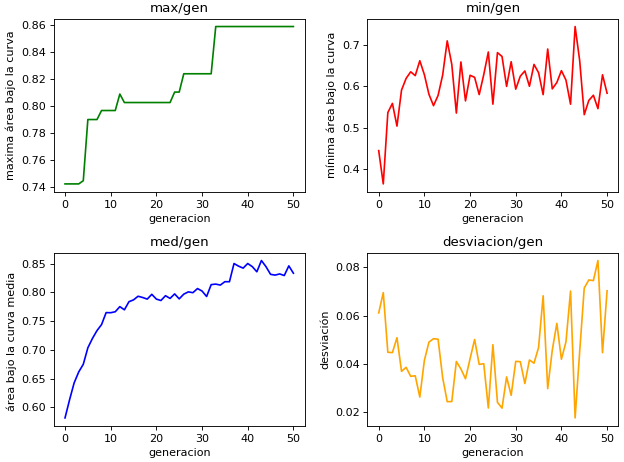
\includegraphics[width=1\textwidth]{images/genetico.png}
    \caption{Gráficas de la evolución de las poblaciones en el algoritmo genético con la métrica=ROC.}
    \label{fig:genetico}
\end{figure}

\subsubsection{Resultados usando Precision-Recall como métrica:} 

Tras la evolución la mayor precisión media que se ha logrado es de 0.1990 con las características indicadas por el individuo [24, 54, 39, 3, 17, 21, 74, 36, 73, 5]. Las características indicadas por el mejor individuo son las siguientes:

\begin{itemize}

    \item \texttt{agg\_linear\_trend} Calcula una regresión lineal de mínimos cuadrados para los valores de las series de tiempo que se agregaron a lo largo de los fragmentos de tamaño 5 en comparación con la secuencia desde 0 hasta el número de fragmentos menos uno. f\_agg="var",attr="intercept".
    \item \texttt{symmetry\_looking} Variable booleana que denota si la distribución es simétrica, con parámetro r=0.6.
    \item \texttt{change\_quantiles} Calcula el promedio del valor absoluto de los cambios consecutivos de la serie entre los cuantiles 0.1 y 0.2. f\_agg="var",isabs=False.
    \item \texttt{change\_quantiles} Entre los cuantiles 0.8 y 0.4. f\_agg="var",isabs=False.
    \item \texttt{change\_quantiles} Entre los cuantilies 0.6 y 0.4. f\_agg="var",isabs=True.
    \item \texttt{last\_location\_of\_minimum} Devuelve la última ubicación del valor mínimo de de la serie.
    \item \texttt{number\_peaks} Calcula el número de picos de al menos anchura 1 en la serie.
    \item \texttt{change\_quantiles} Entre los cuantiles 0.1 y 0.4. f\_agg="mean",isabs=True.
    \item \texttt{change\_quantiles} Entre los cuantiles 1.0 y 0.4. f\_agg="mean",isabs=True.
    \item \texttt{agg\_linear\_trend} Con fragmentos de tamaño 5. f\_agg="min",attr="stderr".
\end{itemize}

En este caso también aparece el mismo atributo (\texttt{change\_quantiles} y \texttt{agg\_linear\_trend}) con distintos parámetros varias veces en el genotipo. 

Por otro lado en la Figura~\ref{fig:genetico2} se aprecia que la primera gráfica (verde), que representa la precisión media del mejor individuo de cada generación, no es estrictamente creciente. Esto puede ocurrir al perder el mejor individuo de la generación al ser mutado o cruzado, sin embargo Deap lleva un histórico de los mejores individuos de cada generación, y al terminar la evolución devuelve el mayor de ellos, no el mejor de la última generación, por lo que el genotipo presentado sí corresponde con el mejor individuo encontrado por el algoritmo genético. 

\begin{figure}
    \centering
    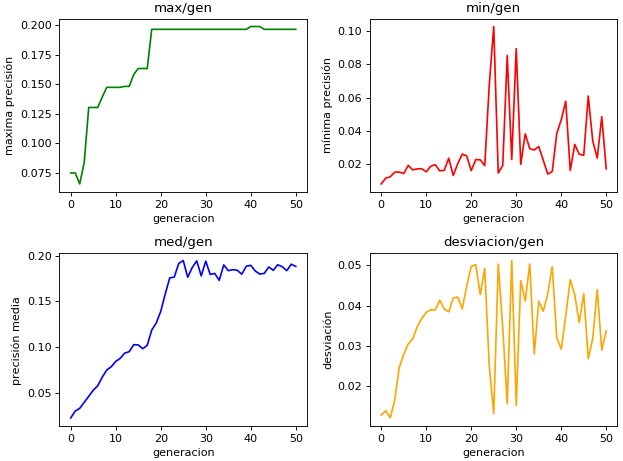
\includegraphics[width=1\textwidth]{images/genetico2.png}
    \caption{Gráficas de la evolución de las poblaciones en el algoritmo genético con la métrica=Precision-Recall.}
    \label{fig:genetico2}
\end{figure}

\chapter{\textit{Ensembles} para desequilibrados \texttt{tsfresh}}
\section{Introducción}
Tras obtener el conjunto de datos que optimiza la curva \textit{Precision-Recall} se han probado diversos \textit{ensembles} para datos desequilibrados. Se han probado tres métodos de remuestreo: \textit{Random Balance}~\cite{diez2015random}, \textit{SMOTE}~\cite{galar2012review} y \textit{Random under sampling}~\cite{diez2015diversity}. Se han usado justo a estos los métodos de \textit{Bagging}~\cite{galar2012review}, \textit{Rotation Forest}~\cite{rodriguez2006rotation} y \textit{RandomCommittee}~\cite{diez2015diversity}. Se ha desechado el uso de métodos de \textit{boosting} ya que los resultados de los experimentos del capítulo~\ref{chap:ensdes} pudimos observar que los datos mal etiquetados afectaban mucho al entrenamiento.

Se ha realizado un entrenamiento con una crisis y testeado con la otra. Se han realizado experimentos utilizando la herramienta Weka~\cite{hall2009weka}. Cada ejemplo se ha ejecutado 10 veces y se ha realizado la media de los resultados. Estos a su vez se han normalizado entre 0 y 1 y son: 
\begin{itemize}
    \item \textbf{TPR}: \textit{True positive rate}
    \item \textbf{FPR}: \textit{False positive rate}
    \item \textbf{TNR}: \textit{True negative rate}
    \item \textbf{FNR}: \textit{False negative rate}
    \item \textbf{PRC}: \textit{Precision-Recall Curve}
    \item \textbf{AUC}: \textit{Area under the ROC Curve}
    \item \textbf{ACC}: \textit{Accuracy}
\end{itemize}

Las abreviaturas para los métodos son:

\begin{itemize}
    \item \textbf{RB}: \textit{Random Balance}
    \item \textbf{RUS}: \textit{Random Undersampling}
    \item \textbf{SM}: \textit{SMOTE}
    \item \textbf{Bag}: \textit{Bagging}
    \item \textbf{RC}: \textit{Random Committee}
    \item \textbf{RotF}: \textit{Rotation Forest}
\end{itemize}

\section{Resultado de experimentos}

Los resultados de entrenar con la primera crisis y testear con la segunda se puede ver en la tabla~\ref{tab:crisis1} y en la figura~\ref{fig:crisis1}. El resultado de la misma operación pero entrenando con la segunda crisis y testeando con la primera está en la tabla~\ref{tab:crisis2} y en la figura~\ref{fig:crisis2}.

\begin{table}\scriptsize
    \begin{center}
        \begin{tabular}{llllllll}
            \toprule
            {} & TPR &          FPR &       TNR & FNR &       PRC &       AUC &       ACC \\
            \midrule
            RB - Bag                &   0 &            0 &         1 &   1 &  0.984425 &  0.552363 &   0.98178 \\
            RB - RC       &   0 &            0 &         1 &   1 &  0.981267 &  0.485675 &   0.98178 \\
            RB - RotF        &   0 &  1.65036e-06 &  0.999998 &   1 &  0.980551 &  0.485354 &  0.981778 \\
            RUS - Bag          &   0 &  0.000899444 &  0.999101 &   1 &  0.980613 &  0.447139 &  0.980897 \\
            RUS - RC &   0 &            0 &         1 &   1 &  0.981076 &    0.4806 &   0.98178 \\
            RUS - RotF  &   0 &  0.000394435 &  0.999606 &   1 &  0.982287 &  0.486412 &  0.981393 \\
            SM - Bag                         &   0 &  0.000173287 &  0.999827 &   1 &  0.984367 &  0.565807 &   0.98161 \\
            SM - RC                &   0 &            0 &         1 &   1 &  0.981278 &  0.486071 &   0.98178 \\
            SM - RotF                 &   0 &  1.56784e-05 &  0.999984 &   1 &  0.982673 &  0.512364 &  0.981764 \\
            \bottomrule
        \end{tabular}
        \caption{Métodos para desbalanceados - Entrenamiento con la primera crisis, testeo con la segunda crisis.}
        \label{tab:crisis1}
    \end{center}
\end{table}

\begin{table}\scriptsize
    \begin{center}
        \begin{tabular}{llllllll}
            \toprule
            {} & TPR &         FPR &       TNR & FNR &       PCR &       AUC &       ACC \\
            \midrule
            RB - Bag                &   0 &   0.0109634 &  0.989037 &   1 &  0.995225 &  0.491511 &  0.983616 \\
            RB - RC       &   0 &  0.00571683 &  0.994283 &   1 &  0.993912 &  0.446135 &  0.988834 \\
            RB - RotF        &   0 &  0.00488364 &  0.995116 &   1 &   0.99517 &  0.525534 &  0.989663 \\
            RUS - Bag          &   0 &   0.0461306 &  0.953869 &   1 &  0.994863 &  0.514533 &  0.948642 \\
            RUS - RC &   0 &   0.0112769 &  0.988723 &   1 &  0.994602 &  0.506568 &  0.983304 \\
            RUS - RotF  &   0 &   0.0128567 &  0.987143 &   1 &  0.994482 &  0.468075 &  0.981733 \\
            SM - Bag                         &   0 &    0.017596 &  0.982404 &   1 &  0.995505 &  0.539099 &   0.97702 \\
            SM - RC                &   0 &   0.0048424 &  0.995158 &   1 &  0.994052 &  0.458383 &  0.989704 \\
            SM - RotF                 &   0 &  0.00344412 &  0.996556 &   1 &  0.994742 &  0.502318 &  0.991094 \\
            \bottomrule
        \end{tabular}
        \caption{Métodos para desbalanceados - Entrenamiento con la segunda crisis, testeo con la primera crisis.}
        \label{tab:crisis2}
    \end{center}
\end{table}

\begin{figure}
    \centering
    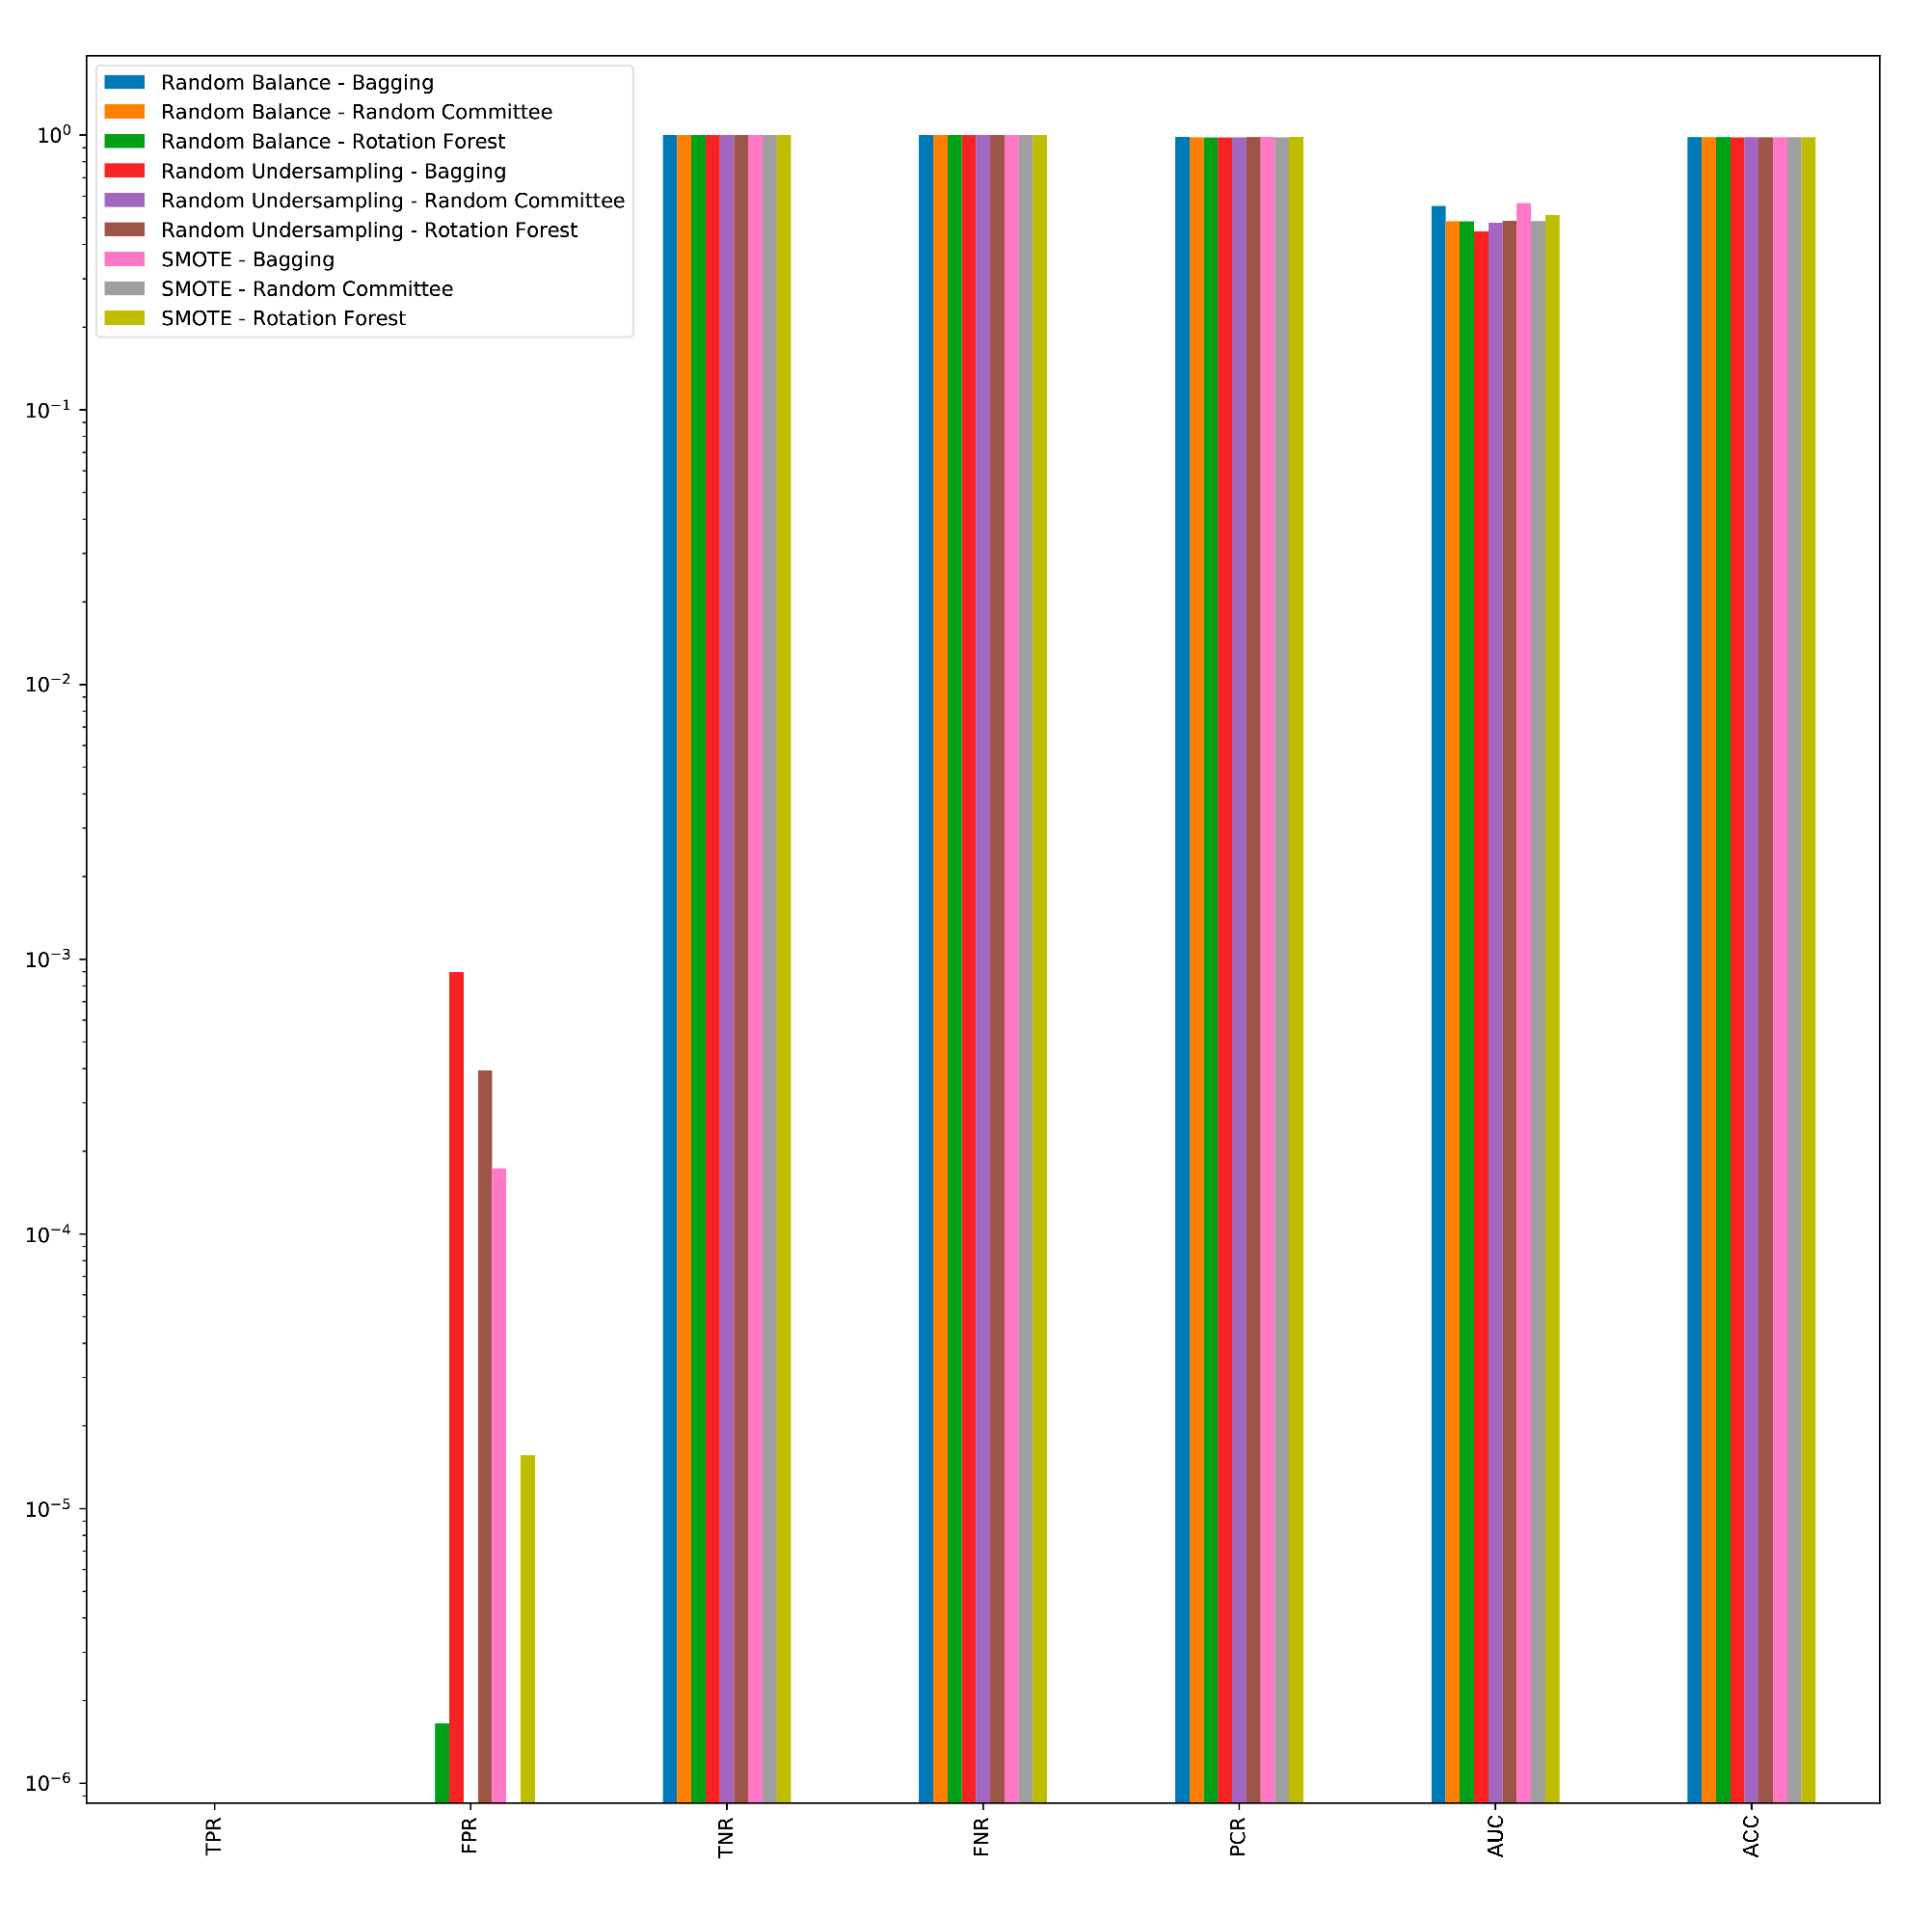
\includegraphics[width=1\textwidth]{images/desbal1.pdf}
    \caption{Métodos para desbalanceados - Entrenamiento con la primera crisis, testeo con la segunda crisis.}
    \label{fig:crisis1}
\end{figure}

\begin{figure}
    \centering
    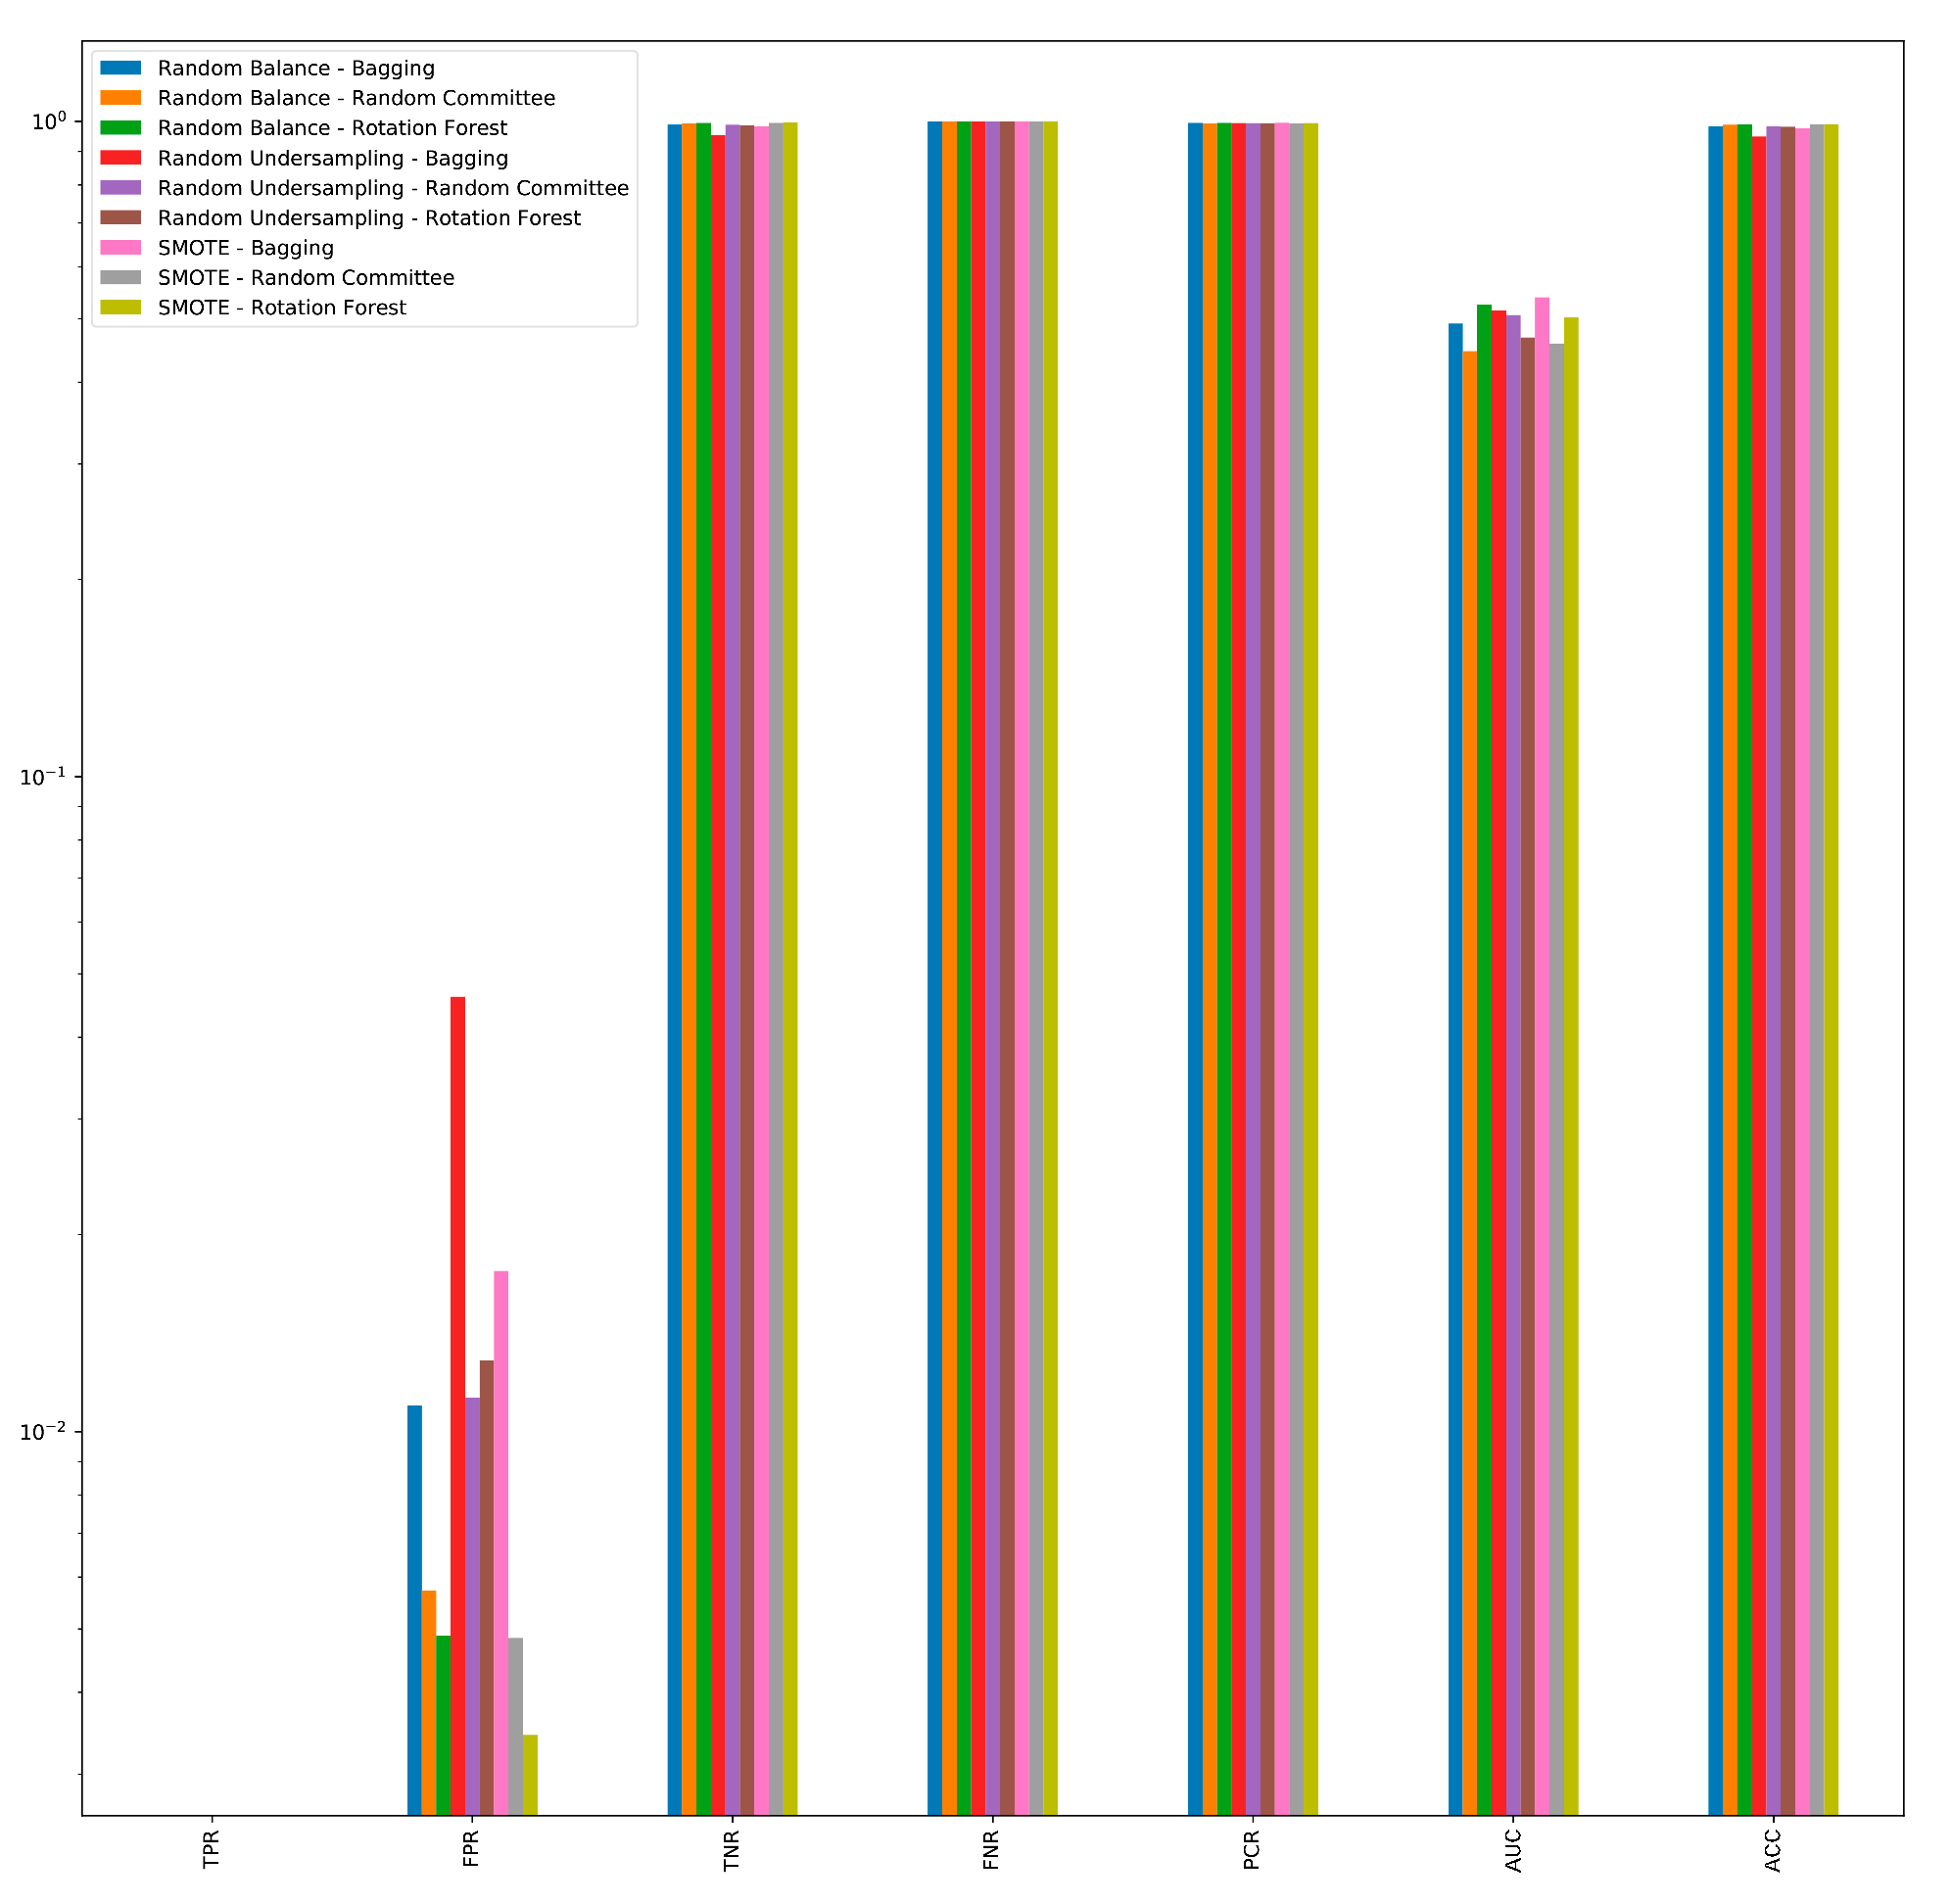
\includegraphics[width=1\textwidth]{images/desbal2.pdf}
    \caption{Métodos para desbalanceados - Entrenamiento con la segunda crisis, testeo con la primera crisis.}
    \label{fig:crisis2}
\end{figure}

\section{Comentario de los resultados}
Como se puede observar gracias a buscar un conjunto de características que optimizan el valor de PRC este valor en todos los experimentos es muy alto. Sin embargo, en todos los experimentos nunca es capaz ningún modelo de predecir correctamente una situación de crisis y las únicas veces que se ha obtenido como resultado de la predicción una situación de crisis han sido erróneas.

A destacar que los métodos que menos error han tenido han sido los que usan \textit{Random Balance} y \textit{SMOTE} y los algoritmos \textit{Rotation Forest} y \textit{Random Committee}.

\section{Conclusiones}
Tras realizar toda esta la investigación e intentar obtener los mejores resultados probando la mayor cantidad técnicas que hemos podido explorar, lamentablemente, debido a la limitación de los datos de crisis y los problemas de como están etiquetados los datos no se ha podido encontrar un modelo que pueda ser usado en producción ya que ningún modelo probado ha sido capaz de predecir correctamente situaciones de crisis. Sin embargo, se espera que si en algún momento se obtuvieran datos suficientes y de calidad, estos mismos experimentos se podrían emplear para encontrar un modelo efectivo. 

\bibliographystyle{plain}
\bibliography{bibliografia}

\end{document}